\documentclass[runningheads]{llncs}
\usepackage[T1]{fontenc}
\usepackage{amsmath,amssymb,mathtools}
\usepackage{array}
\usepackage{booktabs}
\usepackage{graphicx}
\usepackage{float}
\usepackage{tikz}
\usetikzlibrary{arrows.meta,positioning,decorations.pathreplacing}
\usepackage{hyperref}
\hypersetup{hidelinks}
\usepackage{listings}
\lstset{basicstyle=\ttfamily\footnotesize,columns=fullflexible,keepspaces=true,breaklines=true,xleftmargin=2mm,aboveskip=2pt,belowskip=6pt}
\usepackage{microtype}
\usepackage{needspace}
\usepackage{xcolor}

\newif\ifanonymous
\anonymoustrue

\newcommand{\Rocq}{Rocq}
\newcommand{\coqin}[1]{\texttt{#1}}
\newcommand{\PG}{\mathrm{PGL}(2,7)}
\newcommand{\Unif}{U_G}
\newcommand{\worddist}{\mu^{*L}}
\newcolumntype{L}[1]{>{\raggedright\arraybackslash}p{#1}}
\spnewtheorem*{thmAinf}{Theorem A (informal)}{\bfseries}{\itshape}
\spnewtheorem*{thmBinf}{Theorem B (informal)}{\bfseries}{\itshape}
\spnewtheorem*{thmA}{Theorem A}{\bfseries}{\itshape}
\spnewtheorem*{thmB}{Theorem B}{\bfseries}{\itshape}

\title{Algebraic Specification of Card-Based Cryptographic Protocols in Rocq}
\ifanonymous
  \author{Anonymous}
  \institute{Submission to WADT 2026}
\else
  \author{Cheng-Hui Weng}
  \institute{Nagoya University}
\fi

\begin{document}
\maketitle

\begin{abstract}
Card-based protocols use physical cards to compute with information-theoretic
security. I define a \Rocq{} framework with a finite group, its permutation
action, and its shuffle distribution as explicit parameters. The framework
connects group actions with executed traces and word-shuffle mixing. Its main
instance uses the action of $\PG$ on eight projective points. Under the
uniform shuffle distribution, this instance has exact correctness and the
recovery ramp $(t,r,n)=(3,7,8)$, where $t$ is the privacy threshold, $r$ is
the recovery threshold, and $n$ is the number of card positions. It also has
perfect view privacy for coalitions of at most three players. Interpreter
soundness transfers this privacy to executed traces. These privacy results
assume a uniform Boolean secret, a fixed encoded representative, and passive
adversaries. The verifier learns the secret. Active security, security after
the reveal, and composition are outside the model. No single physical move
samples a uniform group element. I therefore analyze a finite implementation
that draws a uniform word of length 200 over five generator letters. A checked
fiber-counting certificate counts the words that evaluate to each group
element. It proves that the resulting word distribution is within $L_1$
distance $2^{-40}$ of the uniform group distribution. The theorem transfers to
single-card marginals and to a product with any secret prior. Transport
theorems then bound approximate coalition-view and executed-trace privacy by
$2^{-39}$ under the word distribution. A five-card family and two related
instances with spectral mixing proofs show which algebraic, operational,
privacy, and mixing arguments the framework reuses. The two spectral instances
import an analytic gap premise, an external assumption used only for their
mixing proofs, as their only assumption beyond the classical principles used
throughout.
\end{abstract}

\section{Introduction}\label{sec:introduction}

Card-based cryptography uses face-down physical cards to compute functions
without computational assumptions. A shuffle hides a permutation. A reveal
exposes selected card faces. Information-theoretic security requires the
resulting observation distribution to hide the protected secret. Den Boer's
five-card protocol computes Boolean conjunction and began this line of
work~\cite{denBoer1989}. Later protocols used fewer cards and supported more
classes of
computations~\cite{MizukiSone2009,MizukiSone2012,KochWalzerHartel2015}.

Mechanized analysis must connect physical operations with their probability
distributions. Koch, Schrempp, and Kirsten use bounded model checking to
search finite protocol spaces and check lower bounds~\cite{Koch2019}. This
method checks a bounded state space, meaning one finite collection of protocol
states. The target class consists of $t$-transitive group actions. A bound for
one such space does not establish a result for all such actions. The Rocq
formalization\footnote{The companion
artifact contains the source, theorem index, assumption report, and build
instructions.}
 instead uses a proof assistant whose generic theorems
quantify over the group, action, and shuffle distribution. It defines reusable
dealer distributions for sampling encoded initial decks, participant views,
and executed traces. The resulting group-parametric model proves perfect trace
privacy. It also checks a word-shuffle mixing bound that connects a finite
generator process with the ideal shuffle law.

The analysis needs two shuffle distributions because the ideal security proof
and the finite implementation use different laws. The uniform distribution on
the shuffle group is the ideal law for the security proofs. No dealer samples
a uniform group element in one physical move. Instead, the dealer repeatedly
draws elementary moves from a small generator alphabet. These draws define the
word distribution over group generators. The physical status of the generator
letters depends on the instance. In the five-card family, the letters are
physical cuts. The $\PG$ letters are group generators, and I do not claim a
physical realization for them. The group parameters connect the two analyses.
Transitivity of the action gives coalition privacy under the ideal law. By
contrast, a small generating alphabet gives a finite executable shuffle whose
word distribution can approximate the ideal law. I first prove security in the
uniform-shuffle model of Section~\ref{sec:model}. I then prove that the word
distribution approximates the uniform law.

I contribute a group-parametric framework. Its primary $\PG$ instance has two
machine-checked security results.

\begin{thmAinf}
For every group element, the $\PG$ instance recovers the secret from all eight
endpoints.\footnotemark 
Under the uniform shuffle distribution, a uniform Boolean
secret, and the fixed representative dealer that always encodes each secret
with its chosen deck, the instance has recovery parameters $(t,r,n)=(3,7,8)$.
It also has perfect view and executed-trace privacy against every passive
coalition of at most three players.
\end{thmAinf}
\footnotetext{Formal statement at the end of
Section~\ref{sec:exact}. The constituent formalized results are
\coqin{pgl27\_run\_recovers}, \coqin{pgl27\_reveal\_ambiguous},
\coqin{pgl27\_seven\_reveal\_class}, \coqin{pgl27\_view\_leak\_k4},
\coqin{pgl27\_view\_indep}, and \coqin{pgl27\_coalition\_trace\_secrecy} in
\path{pgg-smc/instances/pgl27}.}

\begin{thmBinf}
The 200-letter word shuffle over five generator letters is within $L_1$
distance $2^{-40}$ of the uniform shuffle distribution. The fixed
representative dealer uses one chosen deck for each secret. For every passive
coalition of at most three players, the two secret-conditioned view
distributions are within $L_1$ distance $2^{-39}$ of each other. The
corresponding executed coalition-trace distributions satisfy the same bound.
Executed correctness holds for every word.\footnotemark
\end{thmBinf}
\footnotetext{Formal statement at the end of
Section~\ref{sec:mixing}. The constituent formalized results are
\coqin{pgl27\_word\_mixing}, \coqin{pgl27\_word\_view\_indist},
\coqin{pgl27\_word\_trace\_indist}, and \coqin{pgl27\_word\_run\_recovers} in
\path{pgg-smc/instances/pgl27}.}

I make five contributions.
\begin{itemize}
\item I give a common \Rocq{} interface for a finite group, its permutation action,
the shuffle distribution, reconstruction, participant views of the cards held
by a chosen group of players, and executed traces.
\item I verify the den Boer~\cite{denBoer1989} and Kim and
\c{C}etinkaya~\cite{KimCetinkaya2025} five-card protocols in \Rocq{} as one
profile at bias $\varepsilon$, in the sense of Section~\ref{sec:framework}. A
profile packages one instance's data and proofs. I prove executed-run
correctness for the conjunction output, executed-trace privacy against one
corrupted player, and input hiding given the announced output.
\item I prove the exact mutual-information leakage for every reveal pattern in the
five-card family. At bias zero, I recover den Boer's perfect dealing bound. At
bias $1/100$, I kernel-check that after seven cuts every single-card endpoint
distribution is within $L_1$ distance $2^{-40}$ of uniform.
\item For the $\PG$ instance under the uniform shuffle distribution, I prove
correctness and the recovery ramp. The ramp records the privacy threshold, the
recovery threshold, and the number of card positions. I also prove
coalition-view privacy and executed-trace privacy.
\item I prove an $L_1$ bound between a 200-letter word distribution and the
uniform group distribution.\footnote{The $L_1$ distance is
  $\lVert P-Q\rVert_1=\sum_x\lvert P(x)-Q(x)\rvert$, which is called
  variation distance in the formal development, with maximum value 2. The common total
  variation distance is half of it. An $L_1$ bound of $2^{-40}$ therefore
  bounds every observer's distinguishing advantage by $2^{-41}$. The
  paper's security number is the one derived from the coalition-view
  bound: the $2^{-39}$ view distance of Theorem B bounds every observer's
  distinguishing advantage by $2^{-40}$. The $2^{-41}$ figure concerns
  only the group-element mixing distance.} I also transfer this bound to the
distribution of the card at each endpoint and to product distributions with
any secret prior.
\end{itemize}

Section~\ref{sec:model} fixes the protocol flow, the two distributions, and
the security scope. Section~\ref{sec:framework} presents the framework
components used in the proofs. Section~\ref{sec:fivecard} instantiates these
components for the five-card family, whose small deck permits direct case
analysis. Sections~\ref{sec:pgl} and~\ref{sec:exact} construct the $\PG$
instance. Deck enumeration no longer suffices, so three-transitivity carries
the privacy proofs that end in Theorem A. Section~\ref{sec:mixing} proves the
word-shuffle results that end in Theorem B. This section is needed because a
physical dealer repeats elementary moves instead of sampling one uniform group
element. Section~\ref{sec:instances} compares the additional instances and
states the trust base. Section~\ref{sec:related} places the results among
related work. Section~\ref{sec:conclusion} states the remaining extensions and
other future directions.

\section{Protocol and Security Model}\label{sec:model}

A run uses one secret and a deck of face-down cards. The dealer encodes the
secret as a deck arrangement that is valid for the instance. The dealer then
samples a finite-group shuffle and applies its permutation action to the deck.
Each player receives the card at one position. The players reveal their cards
to the verifier. The verifier decodes the secret from the revealed
arrangement. Each instance section depicts this sequence in a flow diagram.

The fixed secret encoding leaves the shuffle as the only source of randomness.
One player observes one card. A coalition view contains the cards at the
coalition's positions. The shuffle distributes each small coalition view
across many deck arrangements. The privacy theorems state exactly that the
resulting coalition-view distribution is independent of the secret. The rest
of this section expresses the same flow as probability distributions.

The framework describes a protocol using the following data:
\begin{equation}
  (G,\rho,\mu;R), \qquad U_G, \qquad \mu^{*L}.
  \label{eq:model-data}
\end{equation}
Here $G$ is a finite shuffle group. The representation $\rho:G\to S_n$ means
that each group element permutes the $n$ card positions. The distribution
$\mu$ selects one generator letter, which denotes one elementary random move.
The real closed field $R$ supplies the probability values. The distribution
$U_G$ is uniform on $G$. I write $\mu^{*L}$ for the word distribution at
length $L$. It is the distribution of the group element obtained by evaluating
$L$ independent letters.

A dealer samples a secret $S$ and a dealt arrangement $D$ that is valid for
the instance. A sampled shuffle $g$ acts on the deck by its permutation action
and produces $\rho(g)D$. Position $i$ of the shuffled arrangement holds the
card that $D$ places at position $\rho(g)(i)$. Player $i$ observes the view
$V_i$ derived from the card at position $i$. A coalition
$C\subseteq\{0,\ldots,n-1\}$ observes the following joint view, which collects
the observations at its named positions:
\begin{equation}
  V_C=(V_i)_{i\in C}.
  \label{eq:coalition-view}
\end{equation}
The interpreter runs the dealer, player, and verifier processes. It records
every value that a process receives. This record is the player's executed
trace $T_i$. For a coalition $C$, the coalition trace $T_C=(T_i)_{i\in C}$
collects the traces of its players. The verifier receives all endpoints and
applies the decoder, which recovers $S$. The verifier therefore learns $S$ by
design.

The following player process makes the execution model concrete by showing the
values that the player receives and reveals\footnote{Formalized in
\path{pgg-smc/protocol/card_exchange_pismc.v} as
\coqin{exchange\_dealer}, \coqin{exchange\_player}, and
\coqin{exchange\_verifier}.}:

\begin{lstlisting}
Definition exchange_player (i : 'I_T)
    : sproc pgg_dtype data (player_idx i) :=
  \pi{ Receive<dealer_idx> #my_hand =>
     Receive<dealer_idx> $shuffle_idx =>
     Reveal<verifier_idx> &(nth ord0 my_hand shuffle_idx) ;
     Finish }.
\end{lstlisting}

In the listing, \coqin{\#} marks a dealt hand, \coqin{\$} marks the public
shuffle index, and \coqin{\&} marks a card position. The player receives the
hand and shuffle index. The player selects one entry and reveals it to the
verifier. The verifier receives this entry as its observation. The interpreter
records the hand and shuffle index in the player's trace. The trace theorem
concerns this process execution. Under the trace-lifting hypothesis, the
recorded trace and the static view determine each other. This is the
interpreter-soundness property used here. The process therefore reveals no
information beyond the static view. Independence of the static view from the
secret consequently gives independence of the executed trace from the secret,
so the proof reuses view privacy.

The primary execution distribution samples a Boolean secret uniformly. For
each secret $s$, it deals one fixed valid deck $D_s$ that represents the class
of $s$. It then applies an independent uniform shuffle. I call this
distribution the fixed representative dealer, and the headline theorems use
it. The all-decks dealer instead samples a valid arrangement uniformly from
the selected secret class before applying the shuffle. Both dealer
distributions use a uniform Boolean prior, so the two secret bits have equal
probability.

The security theorems assume passive, honest-but-curious adversaries. A
corrupted player observes the protocol but does not deviate from it. The
player retains its view and executed trace. Perfect coalition privacy means
that $S$ and $V_C$ are independent. I write
$S\mathrel{\perp}V_C$ for this independence. Perfect trace privacy is stated
by the following equality:
\begin{equation}
  H(S\mid T_C)=H(S).
  \label{eq:trace-privacy}
\end{equation}

The protocol protects a dealt secret, as in a secret-sharing
scheme~\cite{Shamir1979}. The dealer holds the secret. The players hold card
observations that play the role of shares. Privacy limits what coalitions of
curious players learn. The protocol gives the players no private inputs. The
model does not cover active deviation. It also makes no security claim after
the full deck is publicly revealed, and it gives no composition theorem for
multiple executions.

The uniform-shuffle model applies one uniform group element. The word-shuffle
model instead lets the dealer apply a sequence of elementary moves from a
generator alphabet, whose letters name the permitted elementary shuffles. It
replaces $U_G$ with $\mu^{*L}$, the distribution obtained by evaluating $L$
independent letters. I compare distributions $P$ and $Q$ using the $L_1$
distance:
\begin{equation}
  \lVert P-Q\rVert_1=\sum_x\lvert P(x)-Q(x)\rvert.
  \label{eq:l1-definition}
\end{equation}

The word-shuffle model exposes only the product of the word. The dealer
performs 200 physical moves, but no party records an intermediate arrangement.
This non-observation rule is a structural assumption of the formalization. The
dealer process takes a list of alternative cuts and deals one hand for each
cut. Thus a word affects execution only through its evaluated group element.
The uniform-shuffle model uses the same observation rule because its single
uniform shuffle is also unobserved.

Figure~\ref{fig:models} separates the proved paths for the two distributions.
The lower path starts from the finite word distribution and its mixing
certificate. It yields approximate coalition-view and executed-trace privacy
at $2^{-39}$.
\begin{figure}[t]
  \centering
  % Drawn at true document font sizes; the picture is never scaled.
  % It is a little wider than the text block, so it is centred by hand.
  \makebox[\linewidth][c]{%
  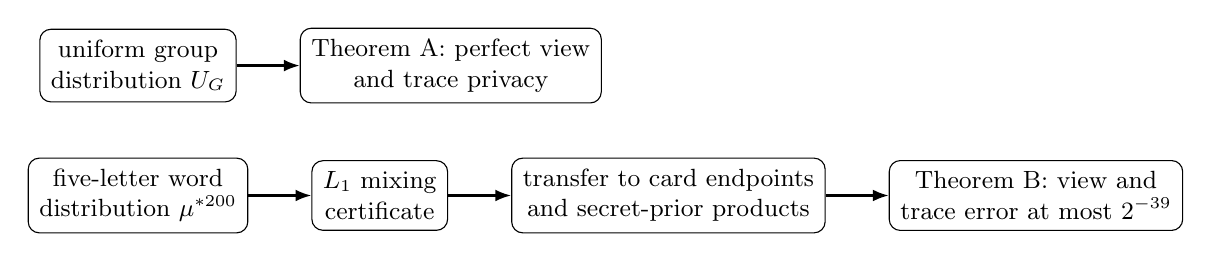
\begin{tikzpicture}[
      node distance=7mm and 8mm,
      box/.style={draw,rounded corners,align=center,inner sep=4pt,
                  font=\small},
      arr/.style={-{Latex[length=2mm]},thick}]
    \node[box] (uniform) {uniform group\\distribution $U_G$};
    \node[box,right=of uniform] (exact) {Theorem A: perfect view\\and trace privacy};
    \draw[arr] (uniform) -- (exact);

    \node[box,below=of uniform] (word) {five-letter word\\distribution $\mu^{*200}$};
    \node[box,right=of word] (lone) {$L_1$ mixing\\certificate};
    \node[box,right=of lone] (transfer) {transfer to card endpoints\\and secret-prior products};
    \node[box,right=of transfer] (privacy)
      {Theorem B: view and\\trace error at most $2^{-39}$};
    \draw[arr] (word) -- (lone);
    \draw[arr] (lone) -- (transfer);
    \draw[arr] (transfer) -- (privacy);
  \end{tikzpicture}}
  \caption{Two proof paths lead to the headline theorems. The upper path ends at Theorem
A. The lower path transfers the mixing certificate from the word distribution
to the view and trace bounds of Theorem B.}
  \label{fig:models}
\end{figure}

\section{Framework and Generic Theorems}\label{sec:framework}

\subsection{Framework Architecture}

Every instance supplies five kinds of data: a group with its action and
generators, a secret type, a run layout, a shuffle-security bound, and a
decoder. I gather these choices in one profile record so that one executable
protocol can be reused across instances. The generic theorems take their
hypotheses directly. I also package the privacy theorem once at the record
level. As a result, a profile with a $t$-transitive action and distinct
encoded decks, meaning that no card value is repeated, inherits privacy for
coalitions of at most $t$ positions. The profile carries the data of
Equation~\ref{eq:model-data} into the executable protocol. The scalar $R$ in
Equation~\ref{eq:model-data} is the real closed field, not a protocol datum.
The finite algebraic structures use Mathematical Components~\cite{MathComp}.
Together, these data and obligations give the record an
algebraic-specification interpretation. The next paragraph develops that
interpretation, and Table~\ref{tab:bridge} then maps each model datum to its
record role and to the values supplied by the $\PG$ instance.

In algebraic specification, the profile record is a parameterized loose
specification. Its fields form the signature, which lists the available data
and operations. Its stated obligations form the axioms that the data must
satisfy. An instance that supplies the fields and proves the obligations is a
model of the specification~\cite{GoguenBurstall1992,SannellaTarlecki2012}.
This interpretation explains the five instances in this paper. Each instance
is a model of the same specification. It also explains the relation between
the ideal and finite shuffle laws. The word-shuffle implementation
approximately refines the uniform-shuffle model, and the $L_1$ bounds of
Section~\ref{sec:mixing} quantify the distance. The formal name invokes
monodromy because one run transports the deal along a group element. Outside
code contexts, I use the term profile record. Because the specification is
loose, it also admits models beyond the five in this paper. Natural next
instances are the affine group $\mathrm{AGL}(1,7)$, which maps any ordered
pair of distinct positions to any other by exactly one element, and
$\mathrm{PGL}(2,11)$ with the present three-transitive parameters. With this
interpretation in place, the following table maps the model data to their
record roles.

\begin{table}[H]
  \centering
  \small
  \begin{tabular}{@{}L{.26\linewidth}L{.36\linewidth}L{.30\linewidth}@{}}
    \toprule
    Model datum & Record role & $\PG$ instance supplies \\
    \midrule
    layout of one protocol run & dealer, player, and verifier processes & eight players, each holding one card \\
    group action $(G,\rho)$ with the generator distribution $\mu$ or the uniform
group distribution $U_G$ & bound on each card position's endpoint distribution under the shuffle law & three-transitive action and a checked bound for the generator-word
distribution \\
    decoder & reconstruction invariant under the group action & orbit-class decoder \\
    run layout, group action and shuffle distribution, and reconstruction & one protocol instance that packages these components & the $\PG$ profile \\
    \bottomrule
  \end{tabular}
  \caption{Mapping from model data to framework records. The source names the run-layout
interface \coqin{PGGInterface}, the shuffle-evidence record
\coqin{SecurityWitness}, the action-compatible reconstruction record
\coqin{ReconPlug}, and the aggregate profile \coqin{MonodromyProfile}.}
  \label{tab:bridge}
\end{table}

The table gives each component's role. Figure~\ref{fig:framework-architecture}
shows the dependencies among the components and auxiliary records. It also
shows how the profile determines the executable protocol.

\begin{figure}[H]
  \centering
  % Drawn at true document font sizes; the picture is never scaled.
  % It is a little wider than the text block, so it is centred by hand.
  \makebox[\linewidth][c]{%
  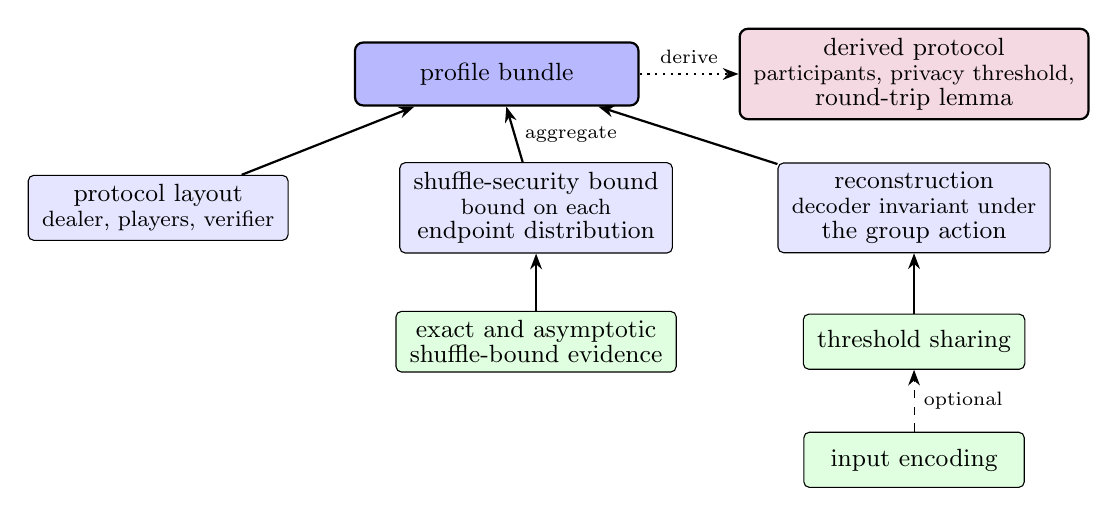
\begin{tikzpicture}[
      every node/.style={font=\small},
      supportbox/.style={
        rectangle, draw, rounded corners=2pt, inner xsep=5pt,
        minimum width=2.8cm, minimum height=0.7cm,
        align=center, fill=green!12
      },
      compbox/.style={
        rectangle, draw, rounded corners=2pt, inner xsep=5pt,
        minimum width=3.2cm, minimum height=0.8cm,
        align=center, fill=blue!10
      },
      bundlebox/.style={
        rectangle, draw, thick, rounded corners=3pt, inner xsep=5pt,
        minimum width=3.6cm, minimum height=0.8cm,
        align=center, fill=blue!28
      },
      derivedbox/.style={
        rectangle, draw, thick, rounded corners=3pt, inner xsep=5pt,
        minimum width=3.6cm, minimum height=0.8cm,
        align=center, fill=purple!15
      },
      arr/.style={-{Stealth[length=2mm]}, thick},
      darr/.style={-{Stealth[length=2mm]}, dashed},
      deparr/.style={-{Stealth[length=2mm]}, dotted, thick}
    ]

    % ===== Bottom: supporting records =====
    \node[supportbox] (ie) at (9.6, 0) {input encoding};
    \node[supportbox] (se) at (4.8, 1.5) {exact and asymptotic\\[-2pt] shuffle-bound evidence};
    \node[supportbox] (ts) at (9.6, 1.5) {threshold sharing};

    % ===== Middle: the three component records =====
    \node[compbox] (pi) at (0, 3.2) {protocol layout\\[-2pt] \footnotesize dealer, players, verifier};
    \node[compbox] (sw) at (4.8, 3.2) {shuffle-security bound\\[-2pt]
      \footnotesize bound on each\\[-2pt] endpoint distribution};
    \node[compbox] (rp) at (9.6, 3.2) {reconstruction\\[-2pt]
      \footnotesize decoder invariant under\\[-2pt] the group action};

    % ===== The aggregate and what it derives =====
    \node[bundlebox] (mp) at (4.3, 4.9) {profile bundle};
    \node[derivedbox] (pr) at (9.6, 4.9) {derived protocol\\[-2pt]
      \footnotesize participants, privacy threshold,\\[-2pt]
      round-trip lemma};

    % ===== Arrows: supporting records into components =====
    \draw[darr] (ie) -- (ts) node[midway, right, font=\scriptsize] {optional};
    \draw[arr] (se) -- (sw);
    \draw[arr] (ts) -- (rp);

    % ===== Arrows: components into the bundle, bundle into the protocol =====
    \draw[arr] (pi) -- (mp);
    \draw[arr] (sw) -- (mp)
      node[midway, right, font=\scriptsize] {aggregate};
    \draw[arr] (rp) -- (mp);
    \draw[deparr] (mp) -- (pr)
      node[midway, above, font=\scriptsize] {derive};
  \end{tikzpicture}}
  \caption{Architecture of the group-parametric card-protocol framework. Blue boxes
denote profile records, green boxes denote auxiliary records, and the purple
box denotes the derived protocol. Solid arrows mark required dependencies. The
dashed arrow marks an optional dependency. The dotted arrow marks derivation.}
  \label{fig:framework-architecture}
\end{figure}

I call a completed profile record a profile. It keeps the participants,
verifier, recovery map that decodes the secret, privacy threshold, and shuffle
bound tied to one instance. Every profile proves three obligations.
\begin{itemize}
\item For every card position, the endpoint-distance field bounds the distance
between that position's post-shuffle card distribution and the uniform
distribution by \coqin{sw\_bound\_eps}. The field is \coqin{sw\_bound}.
\item The threshold scheme provides reconstruction and threshold privacy. The field
\coqin{ts\_correct} decodes every valid share tuple to its secret. The field
\coqin{ts\_private} ensures that every coalition below the threshold sees a
share pattern compatible with each secret in the same way.
\item Reconstruction is invariant under every allowed shuffle. For any valid share
tuple, permuting the shares by the shuffle leaves the recovered secret
unchanged. The field \coqin{rp\_recon\_invariant} states this property.
\end{itemize}

The run layout supplies the executable dealer, player, and verifier processes
described in Section~\ref{sec:model}. The group action and shuffle
distribution determine the dealing rule and endpoint bound. The reconstruction
component selects the decoder. Profiles over the same group can therefore use
different reconstruction schemes.

The security witness records the shuffle distribution and its endpoint bound.
It may record exact evidence, asymptotic evidence, or both.
Table~\ref{tab:witness-mechanism} shows the combinations used by the five
instances. The den Boer row records only exact evidence because one uniform
cut gives the exact endpoint distribution. The $\PG$ row also records only
exact evidence. Section~\ref{sec:mixing} proves the word-shuffle bound of
Theorem~B. This bound is not stored in the record's optional
asymptotic-evidence field. The table therefore reports the record contents,
while the evidence for Theorem~B remains outside the security witness.

\begin{table}[t]
  \setlength{\tabcolsep}{6pt}
  \centering
  \small
  \begin{tabular}{@{}llL{.32\linewidth}L{.20\linewidth}@{}}
    \toprule
    Exact slot & Asymptotic slot & Mechanism & Realized by \\
    \midrule
    present & absent & exact equality of the endpoint and target distributions at $\varepsilon=0$
under the uniform group distribution & den Boer, $\PG$ \\
    present & present & exact finite count giving an error bound that decays geometrically with word
length & Kim \\
    absent & present & spectral certificate based on an imported spectral-gap premise
      & $S_5$ and the direct product $S_5\times S_5$ \\
    \bottomrule
  \end{tabular}
  \caption{Realized combinations of the security witness's two optional evidence fields.
Section~\ref{sec:mixing} gives the word-shuffle counterpart of the $\PG$ row.
Section~\ref{sec:fivecard} proves the den Boer and Kim rows.
Table~\ref{tab:instances} records the evidence for each instance.}
  \label{tab:witness-mechanism}
\end{table}

With an input-encoding component, the flow gains a commit prologue. This phase
collects the players' inputs and assembles the dealt deck, so the flow
computes a function of committed inputs. The realized encoding is den Boer's.
Its orbit obligation places assembled layouts for equal-output inputs in one
shuffle orbit. Thus, it relates different inputs with the same result.
Correctness also requires a valid assembled layout and reconstruction
invariant under every allowed shuffle. These facts imply that the shuffled
layout reconstructs the intended output. The Kim variant reuses the den Boer
program unchanged. With an empty input list, the prologue computes to the
plain dealer used for secret sharing. The $\PG$ instance supplies exactly this
empty list. Section~\ref{sec:fivecard} realizes the committed-input flow. The
instance table in Section~\ref{sec:instances} gives the full comparison.

Section~\ref{sec:fivecard} shows how one instance supplies these components.
Once packaged, the reusable security arguments depend on mathematical
hypotheses, not on the record representation. The next subsection states these
arguments directly.

\subsection{Generic Theorems}

The first generic theorem derives coalition privacy from transitivity. An
instance must provide a $t$-transitive action on decks whose cards are all
distinct. Section~\ref{sec:pgl} proves this requirement for $t=3$.

\begin{theorem}[Generic coalition privacy\footnotemark]\label{thm:generic-privacy}
\footnotetext{Formalized in \path{pgg-smc/reconstruct/transitivity_privacy.v} as
\coqin{ttrans\_view\_indep\_gen}.}
Let $G$ act $t$-transitively on the card positions. Let $S$ be a Boolean
secret with any prior. Suppose that every encoded deck assigns distinct card
values to its positions. If $g$ is uniform on $G$, then 
\[
  S \mathrel{\perp\!\!\!\perp} V_C
\]
 for every
coalition $C$ with $|C|\leq t$.
\end{theorem}

Theorem~\ref{thm:generic-privacy} is also stated once for every profile.
Suppose that the position-permutation group realized by a profile is
$t$-transitive. Suppose also that every encoded deck has distinct cards and
that the profile's share count matches its deck length. Then every coalition
of at most $t$ positions has a view independent of the secret.\footnote{\coqin{profile\_view\_indep} in
\path{pgg-smc/reconstruct/transitivity_privacy.v}, discharged by the $\PG$
instance as \coqin{pgl27\_view\_indep\_via\_profile} in
\path{pgg-smc/instances/pgl27/pgl27_profile_privacy.v}. The derived
corollary restates the instance's view independence verbatim.}
 The
$\PG$ instance proves the first two obligations with its three-transitivity
and distinct-deck lemmas. Both obligations are necessary for the theorem. An
explicit four-position coalition from Section~\ref{sec:pgl} refutes the
conclusion when the coalition bound is weakened to $t+1$. A second profile
over the same group deals one constant card to every position. This
repeated-card encoder leaks the secret to one position, so it refutes the
theorem without the distinct-deck obligation.\footnote{\coqin{profile\_view\_indep\_sharp} and
\coqin{profile\_distinct\_deck\_necessary} in
\path{pgg-smc/instances/pgl27/pgl27_profile_privacy.v}.}
 The record-level
statement retains a two-valued secret. The constant-deck counterexample shows
that distinct cards cannot be omitted. The mathematics therefore excludes the
two-symbol five-card family from this theorem.

Three-transitivity proves privacy for a coalition's card view. The interpreter
instead records an executed trace. The next theorem derives executed-trace
privacy when the trace is determined by the view and the view can be recovered
from the trace.

\begin{theorem}[Generic trace lifting\footnotemark]
\footnotetext{Formalized in \path{pgg-smc/security/pgg_trace_secrecy.v} as
\coqin{trace\_secrecy\_of\_view}.}
Let $S$, $V$, and $T$ be finite random variables. Suppose that $T=\tau(V)$.
Suppose also that a recovery map $\nu$ satisfies $\nu(\tau(v))=v$ for every
$v$. If $V$ is independent of $S$, then 
\begin{equation}
  H(S\mid T)=H(S).
  \label{eq:view-to-trace}
\end{equation}
\end{theorem}

The word-shuffle certificate bounds distributions of group elements. Protocol
security instead concerns card positions after the shuffle, coalition views,
and traces. The next theorem transfers the bound through any deterministic
observable. For a distribution $P$ on $A$, the pushforward $f_*P$ is the
distribution of $f(a)$ when $a$ is sampled from $P$.

\begin{theorem}[Data processing for finite distributions\footnotemark]
\footnotetext{Formalized in \path{pgg-smc/security/pgg_collusion_bound.v} as
\coqin{var\_dist\_fdistmap}.}
Let $P$ and $Q$ be finite distributions on $A$, and let $f:A\to B$. Their
pushforward distributions satisfy 
\[
  \lVert f_*P-f_*Q\rVert_1\leq\lVert P-Q\rVert_1.
\]
\end{theorem}

\section{A First Instance: The Five-Card Family}\label{sec:fivecard}

The five-card family is the simplest concrete instance of the framework. One
profile covers two classic protocols. The cyclic group $C_5$ rotates the
five-card deck, and the decoder tests whether the three hearts are
consecutive. Den Boer's protocol~\cite{denBoer1989} and the Kim and
\c{C}etinkaya variant~\cite{KimCetinkaya2025} differ only in their dealing
distributions. A bias parameter $\varepsilon$ therefore distinguishes them
within the same profile. Figure~\ref{fig:fivecard-run} shows one run.

\begin{figure}[H]
  \centering
  % Drawn at true document font sizes; the picture is never scaled.
  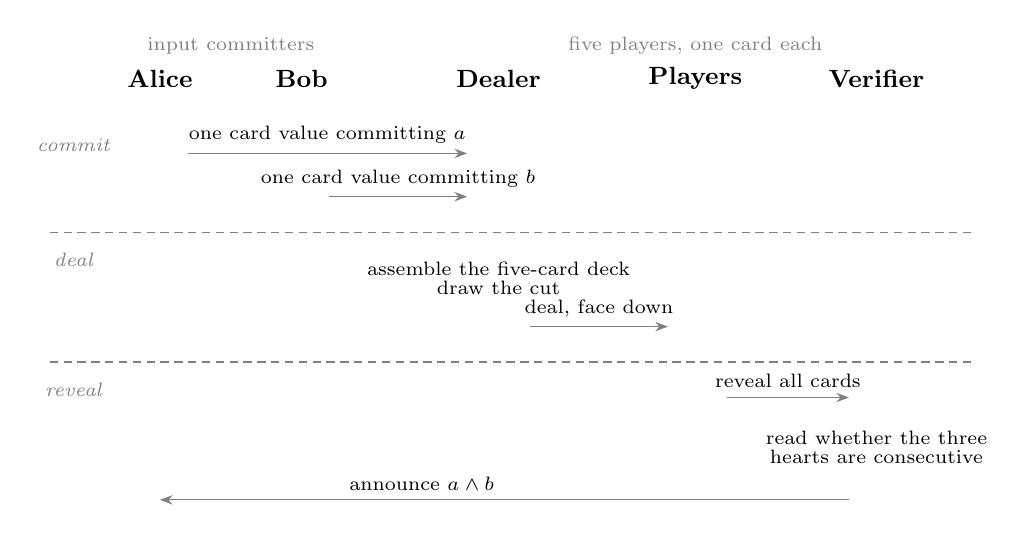
\begin{tikzpicture}[
      partyname/.style={font=\small\bfseries},
      action/.style={font=\scriptsize, align=center},
      msg/.style={-{Stealth[length=1.6mm]}, thin, draw=gray},
      lbl/.style={midway, above, font=\scriptsize},
      phase/.style={font=\scriptsize\itshape, text=gray},
      note/.style={font=\scriptsize, text=gray},
    ]
    % Party headers
    \foreach \x/\name in {1.6/Alice, 3.4/Bob, 5.9/Dealer, 8.4/Players,
                          10.7/Verifier}
      \node[partyname] at (\x, 0) {\name};
    \node[note] at (2.5, 0.42) {input committers};
    \node[note] at (8.4, 0.42) {five players, one card each};

    % Phase: commit
    \node[phase] at (0.5, -0.85) {commit};
    \draw[msg] (1.95, -0.95) -- node[lbl]
      {one card value committing $a$} (5.5, -0.95);
    \draw[msg] (3.75, -1.5) -- node[lbl]
      {one card value committing $b$} (5.5, -1.5);

    % Separator
    \draw[densely dashed, gray] (0.2, -1.95) -- (11.9, -1.95);
    \node[phase] at (0.5, -2.3) {deal};

    \node[action, anchor=north] at (5.9, -2.2)
      {assemble the five-card deck\\[-1pt]draw the cut};
    \draw[msg] (6.3, -3.15) -- node[lbl] {deal, face down} (8.05, -3.15);

    % Separator
    \draw[densely dashed, gray] (0.2, -3.6) -- (11.9, -3.6);
    \node[phase] at (0.5, -3.95) {reveal};

    \draw[msg] (8.8, -4.05) -- node[lbl] {reveal all cards} (10.35, -4.05);
    \node[action, anchor=north] at (10.7, -4.35)
      {read whether the three\\[-1pt]hearts are consecutive};
    \draw[msg] (10.35, -5.35) -- node[lbl, pos=0.62]
      {announce $a\wedge b$} (1.6, -5.35);
  \end{tikzpicture}
  \caption{One five-card run with committed inputs. The physical protocol represents each
input bit with two face-down cards. The formalization represents each
committed bit with one card value.}
  \label{fig:fivecard-run}
\end{figure}

\needspace{5\baselineskip} The five-card family first shows how one profile
combines the framework components. The following definition combines the
cyclic action, the security witness for the biased cut, and the three-hearts
decoder.\footnote{Formalized in
\path{pgg-smc/instances/kim2025/five_card_family.v} as
\coqin{five\_card\_profile}. The listing elides the three bias
hypotheses.}

\begin{lstlisting}
Definition five_card_profile (R : realType) (eps : R)
    (* three bias hypotheses elided *) (L : nat) : MonodromyProfile R :=
  @MkMonodromyProfile R FiveCardKim_M bool FiveCardKim_PI
    (fc_kim_security_witness ... L) (* biased-cut witness    *)
    five_card_plug.                 (* three-hearts decoder  *)
\end{lstlisting}

Kim and \c{C}etinkaya's biased cut defines the dealing distribution. I denote
this distribution by $w_\varepsilon$:
\begin{equation}
  w_\varepsilon(a^k)=\begin{cases}\tfrac{1}{5}-\varepsilon, & k=0,\\[2pt]
  \tfrac{1}{5}+\tfrac{\varepsilon}{4}, & k=1,2,3,4,\end{cases}
  \qquad -\tfrac{4}{5}<\varepsilon<\tfrac{1}{5}.
  \label{eq:fivecard-weight}
\end{equation}
The five weights sum to one. The stated interval makes every weight positive,
so $w_\varepsilon$ is a valid dealing distribution.
At bias zero, the witness bound is zero for every positive word length. In
this precise sense, the unbiased member is den Boer's protocol.\footnote{\coqin{five\_card\_eps0\_eq0} in
\path{pgg-smc/instances/kim2025/five_card_family.v}.}

The reveal-set leakage theorem gives the exact leakage for every fixed reveal
set.\footnote{The master theorem \coqin{leak\_view\_set} covers all
thirty-two position subsets, anchored by \coqin{leak\_k1},
\coqin{leak\_k2\_adj}, \coqin{leak\_k2\_dist2}, \coqin{leak\_k3},
\coqin{leak\_k3\_gap}, \coqin{leak\_k4}, \coqin{leak\_k5}, and the secret's
own entropy \coqin{H\_secret} in
\path{pgg-smc/instances/denboer1989/five_card_leakage.v}. For example
\coqin{leak\_k2\_adj} $=\tfrac{27}{10}-\tfrac14\log 5-\tfrac{7}{10}\log
7$.}
 One revealed card carries no information about the conjunction.
This is the information-theoretic counterpart of the scheme's privacy
threshold. The leakage curve reaches the secret's entropy,
$2-\tfrac34\log 3\approx 0.811$. I call this maximum leakage the cap. The
reported decimals evaluate the proven closed forms.

The leakage values above concern the announced output. The five-card property
in the literature is input-hiding given that output. An observer learns
nothing about the input pair beyond the conjunction that the protocol
announces. The formalization proves this property for every reveal pattern.
Given the announced conjunction, the input pair and the view of any reveal set
are conditionally independent, and their conditional mutual information is
zero.\footnote{\coqin{den\_boer\_cinde} and
\coqin{den\_boer\_input\_private} in
\path{pgg-smc/instances/denboer1989/den_boer_encoding.v}, with the
reveal-set forms \coqin{cinde\_ViewS} and \coqin{input\_private\_ViewS}.}
 Conditioning on the announced output is essential. The view
contains the announcement, so independence fails without this conditioning.

Figure~\ref{fig:fivecard-leakage} shows two features of the leakage theorem.
For two revealed cards, leakage depends on their relative positions. Four and
five revealed cards reach the secret's entropy.

\begin{figure}[H]
  \centering
  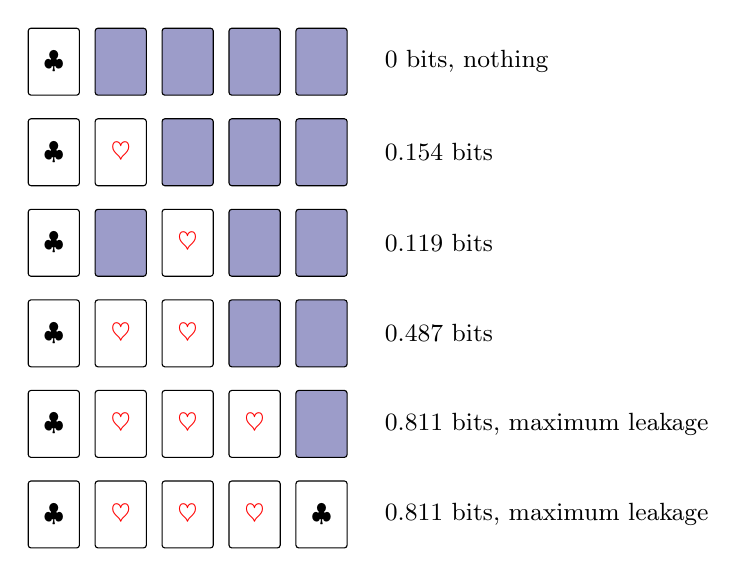
\begin{tikzpicture}[x=8.5mm,y=-11.5mm,
     card/.style={draw,rounded corners=1pt,minimum width=6.5mm,
       minimum height=8.5mm,font=\small},
     down/.style={card,fill=blue!30!gray!60},
     lab/.style={font=\small,anchor=west}]
    \node[card] at (0,1) {$\clubsuit$};
    \node[down] at (1,1) {}; \node[down] at (2,1) {};
    \node[down] at (3,1) {}; \node[down] at (4,1) {};
    \node[lab] at (4.8,1) {$0$ bits, nothing};
    \node[card] at (0,2) {$\clubsuit$};
    \node[card] at (1,2) {\textcolor{red}{$\heartsuit$}};
    \node[down] at (2,2) {}; \node[down] at (3,2) {};
    \node[down] at (4,2) {};
    \node[lab] at (4.8,2) {$0.154$ bits};
    \node[card] at (0,3) {$\clubsuit$};
    \node[down] at (1,3) {};
    \node[card] at (2,3) {\textcolor{red}{$\heartsuit$}};
    \node[down] at (3,3) {}; \node[down] at (4,3) {};
    \node[lab] at (4.8,3) {$0.119$ bits};
    \node[card] at (0,4) {$\clubsuit$};
    \node[card] at (1,4) {\textcolor{red}{$\heartsuit$}};
    \node[card] at (2,4) {\textcolor{red}{$\heartsuit$}};
    \node[down] at (3,4) {}; \node[down] at (4,4) {};
    \node[lab] at (4.8,4) {$0.487$ bits};
    \node[card] at (0,5) {$\clubsuit$};
    \node[card] at (1,5) {\textcolor{red}{$\heartsuit$}};
    \node[card] at (2,5) {\textcolor{red}{$\heartsuit$}};
    \node[card] at (3,5) {\textcolor{red}{$\heartsuit$}};
    \node[down] at (4,5) {};
    \node[lab] at (4.8,5) {$0.811$ bits, maximum leakage};
    \node[card] at (0,6) {$\clubsuit$};
    \node[card] at (1,6) {\textcolor{red}{$\heartsuit$}};
    \node[card] at (2,6) {\textcolor{red}{$\heartsuit$}};
    \node[card] at (3,6) {\textcolor{red}{$\heartsuit$}};
    \node[card] at (4,6) {$\clubsuit$};
    \node[lab] at (4.8,6) {$0.811$ bits, maximum leakage};
  \end{tikzpicture}
  \caption{Mutual-information leakage for selected reveal cases. Blue card backs mark
unrevealed positions. Each value depends only on the revealed positions. The
displayed faces show one possible outcome and do not determine the value.}
  \label{fig:fivecard-leakage}
\end{figure}

Every three-card reveal leaks $\tfrac65-\tfrac{9}{20}\log 3$ bits. The
consecutive and gapped cases therefore have the same value. Only two-card
leakage depends on the relative revealed positions.

\begin{example}\label{ex:fivecard-shape}
Let the reveal expose two of the five positions. Two adjacent positions reveal
$0.154$ bits about the conjunction. Two positions at cyclic distance two
reveal $0.119$ bits. Both decimals evaluate proven closed forms. In
particular, the adjacent value is $\tfrac{27}{10}-\tfrac14\log
5-\tfrac{7}{10}\log 7$. For three revealed cards, the relative positions no
longer affect leakage because the closed form depends only on the number of
revealed cards.
\end{example}

The example describes the information exposed by a fixed reveal set. The
profile also needs a shuffle-security witness for Kim's repeated biased cut.
The next proposition gives this witness at the parameters used here.

\begin{proposition}[Seven-cut security at bias $1/100$\footnotemark]
\label{prop:fivecard-mixing}
\footnotetext{Formalized in
\path{pgg-smc/instances/kim2025/five_card_kim.v} as
\coqin{kim\_bound\_centi} and \coqin{kim\_deal\_centi\_lt}.}
Let the shuffle distribution be the biased cut $w_{1/100}$ repeated seven
times. Then every single-card endpoint distribution is within $L_1$ distance
$2^{-40}$ of uniform.
\end{proposition}

This bound is the profile's quantitative shuffle witness. It measures how
closely one player's card endpoint follows the uniform-cut ideal after seven
biased cuts. The \Rocq{} kernel checks the finite computation.

The two family members share one executed program, so correctness carries over
without change. The Kim program is the den Boer program, and its recovery
theorem reuses the den Boer proof.\footnote{\coqin{kim\_procs} and
\coqin{kim\_run\_recovers} in
\path{pgg-smc/instances/kim2025/kim_run.v}.}
 The committed inputs of the two
players realize the function-evaluation flow of Section~\ref{sec:framework}
with den Boer's input encoding. Den Boer's uniform cut gives the exact
endpoint distribution after one shuffle. For one corrupted player, the
executed trace leaves the secret's conditional entropy equal to its plain
entropy.\footnote{\coqin{kim\_trace\_secrecy} in
\path{pgg-smc/instances/kim2025/kim_trace.v}.}
 Table~\ref{tab:instances} in Section~\ref{sec:instances}
gives the full comparison.

The five-card family uses a cyclic group and a deck small enough for kernel
enumeration. The next sections instantiate the same records when enumeration
is not feasible. The $\PG$ construction strengthens coalition privacy beyond
one card by using three-transitivity and an orbit-class secret. Its word
certificates avoid computation inside the group.

\section{The \texorpdfstring{$\PG$}{PGL(2,7)} Construction}\label{sec:pgl}

I construct the paper's main eight-player instance in this section. It is an
instance of the profile specification, which packages the data and proof
obligations for one protocol instance. The construction supplies the record
fields of Section~\ref{sec:framework} and proves their obligations. Each
player receives one card as a physical share of the secret. Under the fixed
representative dealer and an independent uniform $\PG$ shuffle, every passive
coalition of at most three players has perfect view and executed-trace
privacy. Every reveal of seven positions determines the secret class. Every
reveal of at most six positions remains compatible with both classes. A view
of four positions can leak information, so the privacy cutoff at three is
sharp. These thresholds give the recovery ramp $(t,r,n)=(3,7,8)$. Decoding the
full eight-card arrangement is correct for every allowed group element.
Theorem~A collects these exact guarantees. Theorem~B later replaces the
uniform group element with a uniformly sampled 200-letter generator word and
bounds the resulting privacy error. To build the instance that supports these
results, I first specify its eight card positions.

I index the eight card positions by the projective line over $\mathbb{F}_7$,
which consists of seven field elements and one point at infinity:
\[
  X=\mathbb{P}^1(\mathbb{F}_7)=\{0,1,\ldots,6,\infty\}.
\]
The symbols $0,\ldots,6$ are the seven field elements. The symbol $\infty$ is
the additional projective point. Each point labels one physical position and
the player who receives its card. Card values use the separate labels
$C=\{0,1,\ldots,7\}$. Thus all eight cards carry distinct symbols. This
standard-deck setting uses pairwise distinguishable cards of the kind found in
common decks. Most protocol sizes are instead measured for two-symbol
encodings~\cite{NiemiRenvall1999,Koch2019}. The group $G=\PG$ acts on $X$ by
fractional linear transformations. Each group element therefore permutes the
eight card positions and defines an allowed deck rearrangement. The group has
order\footnote{Formalized in
\path{pgg-smc/instances/pgl27/pgl27_mixing.v} as \coqin{pgl27\_card}. The
order of the abstract quotient is \coqin{pgl27\_pgl2\_order} in
\path{pgg-smc/instances/pgl27/pgl27_group.v}.}:
\begin{equation}
  \lvert G\rvert=336.
  \label{eq:pgl-order}
\end{equation}
The formal representation assigns the point at infinity $\infty$ to position
seven.

The $\PG$ action on $X$ also moves sets of four card positions by moving every
position in the set. I encode the secret bit as the orbit class of the four
positions occupied by hearts. Every allowed shuffle keeps this set in the same
orbit, so the orbit label does not change. This invariance gives correctness
under shuffling. Privacy requires a separate argument about the card values
that a coalition sees at its named positions.

\subsection{Orbit Encoding of the Secret}

I make the encoding precise in four steps. First, I define the four-position
heart patterns obtained from valid decks under allowed shuffles. Next, I give
an explicit classifier for the two orbits. I then choose one deck from each
class. Finally, I prove that every allowed shuffle preserves the classifier.

\begin{definition}[Orbit of four positions]
Let $\Omega_4$ be the set of all four-position subsets of $X$: \[
\Omega_4=\{A\subseteq X\mid |A|=4\}. \] For $A,B\in\Omega_4$, define the orbit
and orbit equivalence by \[ \operatorname{Orb}_G(A)=\{g\mathbin{\cdot}A\mid
g\in G\}, \qquad A\sim_G B \quad\Longleftrightarrow\quad
B\in\operatorname{Orb}_G(A). \]
\end{definition}

Each set $A\in\Omega_4$ records the four positions occupied by hearts but
forgets the individual labels of those four hearts. In this subsection, every
orbit is an orbit in $\Omega_4$. Two heart-position patterns are equivalent
when an allowed group action carries one to the other. Each valid labelled
deck therefore selects one orbit representative, namely its concrete set of
heart positions.

To decode an orbit label from a deck, I first extract the heart positions. I
then need a test whose value is constant within each orbit and differs between
the two orbits. The cross ratio supplies this test.

\begin{definition}[Heart-position map and decoder\footnotemark]
\footnotetext{Formalized in
\path{pgg-smc/instances/pgl27/pgl27_orbit.v} as
\coqin{is\_heart}, \coqin{deck\_ok}, \coqin{heart\_set},
\coqin{cross\_ratio}, \coqin{equianharmonic}, \coqin{subset\_class}, and
\coqin{orbit\_class}.}
A valid deck is a bijection $D:X\to C$. Its four heart-labeled card values are
$0,1,2,3$. Their positions form 
\[
  H(D)=\{i\in X\mid D(i)\in\{0,1,2,3\}\}\in\Omega_4.
\]
 Let $A=\{a<b<c<d\}$ under the order
$0<1<\cdots<6<\infty$. Define the cross ratio in the finite field
$\mathbb{F}_7$ by 
\[
  [a,b;c,d]=\frac{(a-c)(b-d)}{(a-d)(b-c)},
  \qquad
  [a,b;c,\infty]=\frac{a-c}{b-c}.
\]
 The second formula covers the projective point at
infinity. Because the four points are distinct, their cross ratio is neither
zero nor one. The five listed values therefore exhaust the possible elements
of $\mathbb{F}_7$. Define the classifier
$\kappa:\Omega_4\to\{0,1\}$ by 
\[
  \kappa(A)=
  \begin{cases}
    1, & [a,b;c,d]\in\{3,5\},\\
    0, & [a,b;c,d]\in\{2,4,6\}.
  \end{cases}
\]
 The
classifier maps the equianharmonic class to one and the harmonic class to
zero. The deck decoder is 
\[
  \operatorname{dec}(D)=\kappa(H(D)),
  \qquad
  D\xmapsto{H}\Omega_4\xmapsto{\kappa}\{0,1\}.
\]
\end{definition}

For $\kappa$ to be an orbit label, each fiber of $\kappa$ must equal one orbit
of $G$. A fiber is the set of patterns assigned one classifier value. Thus
$\kappa$ must be constant on each orbit and must give different values to
distinct orbits. The next theorem proves both requirements and counts the two
fibers.

\begin{theorem}[The two orbit classes\footnotemark]
\label{thm:orbit-split}
\footnotetext{Formalized in
\path{pgg-smc/instances/pgl27/pgl27_orbit.v} as
\coqin{subset\_class\_orbit}, \coqin{subset\_class\_orbitE},
\coqin{orbit\_class\_split}, and
\coqin{orbit\_class\_split\_complement}.}
For all $A,B\in\Omega_4$, 
\[
  \kappa(A)=\kappa(B)
  \quad\Longleftrightarrow\quad
  \exists g\in G,\ B=g\mathbin{\cdot}A.
\]
 Thus the quotient by orbit equivalence
has two classes: 
\[
  \Omega_4/G\cong\{0,1\},
  \qquad
  |\kappa^{-1}(0)|=42,
  \qquad
  |\kappa^{-1}(1)|=28.
\]
 The fiber $\kappa^{-1}(0)$ is harmonic. The fiber
$\kappa^{-1}(1)$ is equianharmonic.
\end{theorem}

I use the two stable orbit labels to represent a Boolean secret. For each
label $s\in\{0,1\}$, the dealer fixes one valid representative deck $D_s$. The
dealer later shuffles this deck and gives one card to each player. Orbit
invariance will prove correctness. Privacy will follow later from the shuffle
distribution and three-transitivity, which makes each ordered observation of
at most three positions uniform. The following definition gives the two
representative decks and the encoder.

\begin{definition}[Orbit encoder\footnotemark]
\footnotetext{Formalized in
\path{pgg-smc/instances/pgl27/pgl27_orbit.v} as
\coqin{orbit\_encode} and \coqin{orbit\_encode\_deck}.}
For each secret $s\in\{0,1\}$, let $D_s$ be a valid representative deck
whose heart-position set has orbit label $s$. In this instance, take
\[
  D_0=(0,1,2,3,4,5,6,7),
  \qquad
  D_1=(0,1,2,4,3,5,6,7),
\]
and define the encoder by $\operatorname{enc}(s)=D_s$.
\end{definition}

Figure~\ref{fig:encoding} shows the different heart-position patterns in the
two representative decks.

\begin{figure}[H]
  \centering
  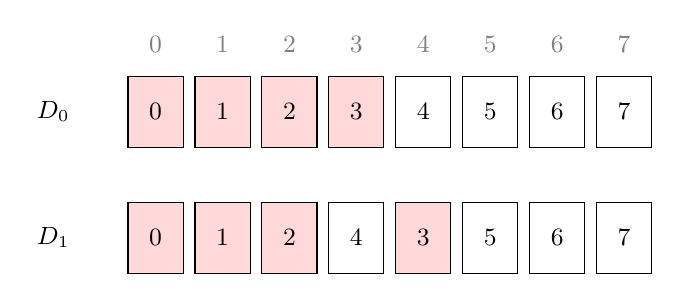
\begin{tikzpicture}[every node/.style={font=\small},
      card/.style={draw,minimum width=7mm,minimum height=9mm,inner sep=1pt},
      heart/.style={card,fill=red!15}]
    \node at (-1.3,0) {$D_0$};
    \foreach \p/\c/\s in {0/0/heart,1/1/heart,2/2/heart,3/3/heart,
                          4/4/card,5/5/card,6/6/card,7/7/card}
      \node[\s] at (\p*0.85,0) {$\c$};
    \node at (-1.3,-1.6) {$D_1$};
    \foreach \p/\c/\s in {0/0/heart,1/1/heart,2/2/heart,3/4/card,
                          4/3/heart,5/5/card,6/6/card,7/7/card}
      \node[\s] at (\p*0.85,-1.6) {$\c$};
    \foreach \p in {0,...,7}
      \node[gray] at (\p*0.85,0.85) {\p};
  \end{tikzpicture}
  \caption{The two encoded representatives. Gray labels mark card positions, and position
seven represents $\infty$. Boxed numbers are card values. Shading marks the
four heart-labeled card values. The row $D_0$ represents the harmonic secret
$0$. The row $D_1$ represents the equianharmonic secret $1$.}
  \label{fig:encoding}
\end{figure}

The decoder must assign each representative deck to the bit that its encoder
received. The following calculation checks this encoder-decoder round trip for
both representatives. Shuffle invariance will then extend the equality to
every deck reachable from either representative.

\begin{example}[Decoding the representatives\footnotemark]
\footnotetext{Formalized in
\path{pgg-smc/instances/pgl27/pgl27_orbit.v} as
\coqin{orbit\_encodeK}.}
The rows in Figure~\ref{fig:encoding} satisfy 
\[
  H(D_0)=\{0,1,2,3\},
  \qquad
  \kappa(H(D_0))=0,
\]
 and 
\[
  H(D_1)=\{0,1,2,4\},
  \qquad
  \kappa(H(D_1))=1.
\]
 Thus
the complete encoding path applies the encoder, heart-set extraction, and
classifier in order: 
\[
  s\longmapsto D_s
   \longmapsto H(D_s)
   \xmapsto{\kappa}s,
  \qquad
  \operatorname{dec}(\operatorname{enc}(s))=s.
\]
\end{example}

The example proves $\operatorname{dec}(\operatorname{enc}(s))=s$ before
shuffling. Correctness of a full run also requires the decoder to return the
same value after every allowed shuffle. Let $\rho:G\to S_X$ be the permutation
of card positions induced by the group action. A deck $D:X\to C$ maps each
position to its card value. Define the shuffled deck by:
\[
  (g\star D)(i)=D(\rho(g)(i)).
\]
The symbol $\star$ denotes this deck rearrangement. In $g\star D$, position
$i$ contains the value that $D$ places at $\rho(g)(i)$. The set of new heart
positions therefore pulls the old heart set back through $\rho(g)$, which
produces the inverse position action. The following lemma states this
heart-set transport.

\begin{lemma}[Shuffle invariance\footnotemark]
\footnotetext{Formalized in
\path{pgg-smc/instances/pgl27/pgl27_orbit.v} as
\coqin{subset\_class\_invariant}, \coqin{orbit\_class\_invariant}, and
\coqin{deck\_stable}. The heart-set identity is the local equality
\coqin{Hheart} in the proof of \coqin{orbit\_class\_invariant}, not a
separate exported theorem.}
For every $g\in G$ and valid deck $D$, the heart positions move by the inverse
positional action: 
\[
  H(g\star D)=\rho(g)^{-1}\mathbin{\cdot}H(D).
\]
 The shuffled deck remains valid, and its decoded
value does not change: 
\[
  g\star D\text{ is valid},
  \qquad
  \operatorname{dec}(g\star D)=\operatorname{dec}(D).
\]
\end{lemma}

The equality $\rho(g)^{-1}=\rho(g^{-1})$ shows that the inverse permutation
comes from the inverse group element. Thus the shuffled heart set remains in
the same $G$-orbit as $H(D)$. The shuffle may change the orbit representative
in $\Omega_4$, but the orbit label remains fixed.

In one run, the dealer encodes $s$ as $D_s$, applies an allowed shuffle, and
gives one card to each player. When all eight players reveal their cards, the
verifier sees $g\star D_s$. Proposition~\ref{thm:pgl-correctness} later lifts
deck-level correctness to the executable interpreter. The recovery threshold
asks how many revealed positions determine the secret. Coalition privacy asks
what smaller named groups learn. Section~\ref{sec:exact} proves these two
separate properties. Those later arguments depend first on deck-level
correctness. The following corollary states the equality required by this
execution.

\begin{corollary}[Shuffle correctness of orbit decoding\footnotemark]
\label{cor:orbit-shuffle-correctness}
\footnotetext{The direct equality is formalized in
\path{pgg-smc/instances/pgl27/pgl27_orbit.v} as
\coqin{orbit\_encodeK} and \coqin{orbit\_class\_invariant}. The
reconstruction-interface counterpart is
\coqin{orbit\_recon\_invariant} in
\path{pgg-smc/instances/pgl27/pgl27_scheme.v}.}
For every $s\in\{0,1\}$ and $g\in G$, 
\[
  \operatorname{dec}(g\star\operatorname{enc}(s))
  =\operatorname{dec}(\operatorname{enc}(s))
  =s.
\]
\end{corollary}

Corollary~\ref{cor:orbit-shuffle-correctness} shows that every allowed shuffle
preserves the decoded secret of an encoded deck. Correctness and privacy
require separate arguments. Privacy concerns the distribution of partial
observations when $g\leftarrow U_G$ is uniform and independent of the secret.
A coalition's partial observation contains only the card values at its named
positions. The privacy proof uses three-transitivity, which lets the action
carry any ordered triple of distinct positions to any other. Before I give
that proof, I use the next figure to return from the deck equality to one
complete execution.

Figure~\ref{fig:run} shows where the encoder and decoder act during one
execution.

\begin{figure}[H]
  \centering
  % Drawn at true document font sizes; the picture is never scaled.
  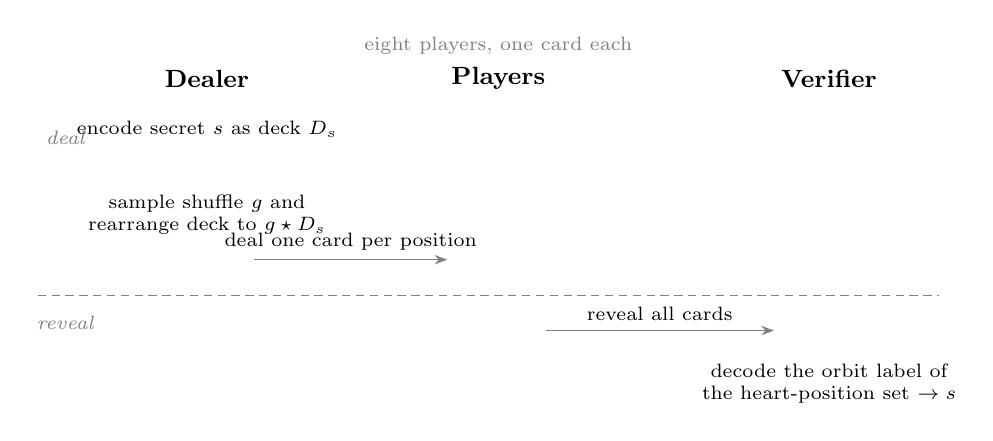
\begin{tikzpicture}[
      partyname/.style={font=\small\bfseries},
      action/.style={font=\scriptsize, align=center},
      msg/.style={-{Stealth[length=1.6mm]}, thin, draw=gray},
      lbl/.style={midway, above, font=\scriptsize},
      phase/.style={font=\scriptsize\itshape, text=gray},
      note/.style={font=\scriptsize, text=gray},
    ]
    % Party headers
    \foreach \x/\name in {2.3/Dealer, 6.0/Players, 10.2/Verifier}
      \node[partyname] at (\x, 0) {\name};
    \node[note] at (6.0, 0.42) {eight players, one card each};

    % Phase: deal
    \node[phase] at (0.5, -0.75) {deal};
    \node[action, anchor=north] at (2.3, -0.42)
      {encode secret $s$ as deck $D_s$};
    \node[action, anchor=north] at (2.3, -1.35)
      {sample shuffle $g$ and\\rearrange deck to $g\star D_s$};
    \draw[msg] (2.9, -2.3) -- node[lbl]
      {deal one card per position} (5.35, -2.3);

    % Separator
    \draw[densely dashed, gray] (0.15, -2.75) -- (11.6, -2.75);
    \node[phase] at (0.5, -3.1) {reveal};

    \draw[msg] (6.6, -3.2) -- node[lbl] {reveal all cards} (9.5, -3.2);
    \node[action, anchor=north] at (10.2, -3.5)
      {decode the orbit label of\\the heart-position set $\to s$};
  \end{tikzpicture}
  \caption{One $\PG$ run with eight players and one card per player. The players supply
no private inputs. The verifier decodes the orbit label of the heart-position
set. In the uniform-shuffle model, $g$ follows the uniform distribution $U_G$.
In the word-shuffle model, $g$ follows the word distribution $\worddist$. This
run is the no-input counterpart of Figure~\ref{fig:fivecard-run}.}
  \label{fig:run}
\end{figure}

\subsection{Action and Generators}

The protocol uses the permutation action $\rho:G\to S_X$ on the eight card
positions. A generator is one element of a fixed set whose finite products
reach every element of $G$. Under $\rho$, each generator rearranges the eight
cards once. A generator word lists a sequence of these elementary
rearrangements. Evaluating the word gives its product $g\in G$. In the passive
execution model, no party observes an intermediate arrangement. The word
therefore affects execution only through $g$ and the final deck $g\star D_s$.

For $G=\PG$, three fractional linear transformations generate the group.
Translation is $z\mapsto z+1$. Scaling is $z\mapsto 3z$. Inversion is
$z\mapsto -1/z$.\footnote{The rows of Figure~\ref{fig:pgl-generators} are
the permutation tables of the three maps, identified with them by
\coqin{tr\_moebius}, \coqin{sc\_moebius}, and \coqin{inv\_moebius} in
\path{pgg-smc/instances/pgl27/pgl27_group.v}.}
 On the projective line, translation and scaling fix
$\infty$, while inversion exchanges $0$ and $\infty$.
Figure~\ref{fig:pgl-generators} shows each map as a rearrangement of eight
cards, one at each projective point. The five-letter alphabet used by the
executable shuffle in Section~\ref{sec:mixing} adds the inverses of
translation and scaling to these three maps. The group order is
$|G|=336=8\cdot7\cdot6$, which is also the number of ordered triples of
distinct points. Lemma~\ref{thm:three-transitive} provides a group element for
each ordered destination triple. The count then makes this element unique.

\begin{figure}[t]
  \centering
  % Drawn at true document font sizes; the picture is never scaled.
  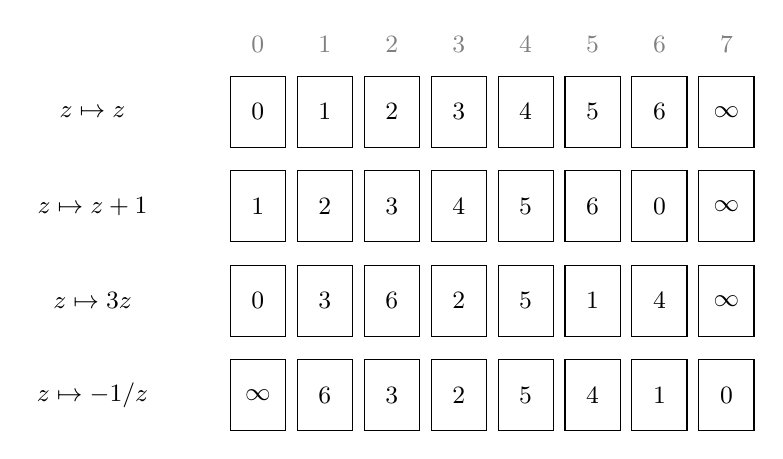
\begin{tikzpicture}[every node/.style={font=\small},
      card/.style={draw,minimum width=7mm,minimum height=9mm,inner sep=1pt}]
    \foreach \p in {0,...,7}
      \node[gray] at (\p*0.85,0.85) {\p};
    \node at (-2.1,0) {$z\mapsto z$};
    \foreach \p/\c in {0/0,1/1,2/2,3/3,4/4,5/5,6/6,7/\infty}
      \node[card] at (\p*0.85,0) {$\c$};
    \node at (-2.1,-1.2) {$z\mapsto z+1$};
    \foreach \p/\c in {0/1,1/2,2/3,3/4,4/5,5/6,6/0,7/\infty}
      \node[card] at (\p*0.85,-1.2) {$\c$};
    \node at (-2.1,-2.4) {$z\mapsto 3z$};
    \foreach \p/\c in {0/0,1/3,2/6,3/2,4/5,5/1,6/4,7/\infty}
      \node[card] at (\p*0.85,-2.4) {$\c$};
    \node at (-2.1,-3.6) {$z\mapsto -1/z$};
    \foreach \p/\c in {0/\infty,1/6,2/3,3/2,4/5,5/4,6/1,7/0}
      \node[card] at (\p*0.85,-3.6) {$\c$};
  \end{tikzpicture}
  \caption{The three generating maps on the projective points. Each row shows one
elementary group transformation. Gray labels mark positions. The box at
position $i$ contains its image point $g(i)$. Position seven represents
$\infty$.}
  \label{fig:pgl-generators}
\end{figure}

The figure gives the three permutation tables. The following example first
reads each table as a physical movement of the card row. It then shows how a
generator word sends one ordered triple of source points to an ordered triple
of target points.

\begin{example}\label{ex:pgl-letters}
Start with the identity row, which places label $z$ at position $z$.
Translation changes $(0,1,2,3,4,5,6,\infty)$ to $(1,2,3,4,5,6,0,\infty)$
because position $i$ displays $g(i)$. Scaling fixes $0$ and $\infty$. It
cycles the other six points in one six-cycle. Inversion is an involution, so
applying it twice gives the identity. It exchanges $0$ with $\infty$, $1$ with
$6$, $2$ with $3$, and $4$ with $5$. Words in these three maps reach all $336$
group elements. Lemma~\ref{thm:three-transitive} gives one such word for every
ordered triple of distinct points. For example, apply inverse scaling, inverse
translation, inversion, scaling, and inverse translation in that order. This
five-letter generator word evaluates to $z\mapsto(z-1)/(3-z)$ and sends
$(0,1,2)$ to $(2,0,1)$.
\end{example}

\subsection{Three-Transitivity and Local Views}

The action of $\PG$ on the eight projective points is sharply
three-transitive. Thus exactly one group element sends any ordered triple of
distinct points to any other. The uniqueness follows because the group order
is $336=8\cdot7\cdot6$, which is the number of ordered triples. Under a
uniform shuffle, every ordered view of three positions is uniform and carries
no group invariant. A view of four positions carries one invariant, the cross
ratio. This algebraic fact has four consequences. It makes the cross-ratio
decoder possible. It gives perfect privacy to coalitions of at most three
players. It forces coalitions of four players to leak information. It also
explains the choice of $\PG$ for the construction.

Global orbit invariance proves correctness. Privacy asks what card values a
fixed coalition sees when $g\leftarrow U_G$ is independent and uniform. The
coalition observes named positions, so an ordered tuple must preserve which
player saw each value.

\begin{lemma}[Three-transitivity\footnotemark]\label{thm:three-transitive}
\footnotetext{Formalized in \path{pgg-smc/instances/pgl27/pgl27_group.v} as
\coqin{pgl27\_3transitive}.}
For any ordered triples $(x_1,x_2,x_3)$ and $(y_1,y_2,y_3)$ of distinct
projective points, there exists $g\in\PG$ such that 
\[
  g(x_1)=y_1,
  \qquad
  g(x_2)=y_2,
  \qquad
  g(x_3)=y_3.
\]
\end{lemma}

The formal proof enumerates generator words from one fixed base triple to
every distinct target triple. The Rocq kernel checks the resulting finite
table. The base triple is $(0,1,2)$. For every other ordered triple of
distinct points, the table stores one generator word that sends $(0,1,2)$ to
that triple. Lemma~\ref{thm:three-transitive} then makes every ordered view of
at most three positions uniform under $U_G$. This lemma supplies the
group-action premise of Theorem~\ref{thm:generic-privacy} at $t=3$. The
generic theorem gives uniform-shuffle coalition privacy.
Section~\ref{sec:mixing} treats the nonuniform word distribution separately
because it requires a mixing argument.

Table~\ref{tab:source-index} at the end of Section~\ref{sec:mixing} lists the
formal source locations for this section and the next two sections.

\section{Correctness, Recovery, and Uniform-Shuffle Privacy}\label{sec:exact}

The construction section proved deck-level correctness and the group-action
condition needed for privacy. This section lifts correctness from decks to
full protocol executions. It also determines the recovery ramp and proves view
and trace privacy under a uniform shuffle. Together, these results form
Theorem A.

\subsection{Correctness and Recovery}

The interpreter deals $D_s$, applies an allowed shuffle, and sends one card to
each of eight players.\footnote{The dealer program is
\coqin{exchange\_dealer} and the $\PG$ witness is the singleton cut list in
\coqin{pgl27\_dealer\_run}.}
 The players return their cards to the
verifier. The verifier's endpoint sequence is the shuffled dealt arrangement.
Orbit-class invariance and the encoder equation, which identifies the decoded
orbit class with the encoded secret, then prove correctness.

\begin{proposition}[Executed correctness\footnotemark]\label{thm:pgl-correctness}
\footnotetext{Formalized in \path{pgg-smc/instances/pgl27/pgl27_run.v} as
\coqin{pgl27\_run\_recovers}. The direct class-recovery counterpart is
formalized in \path{pgg-smc/instances/pgl27/pgl27_trace.v} as
\coqin{pgl27\_run\_recovers\_class}.}
\par
For every $s\in\{0,1\}$ and $g\in\PG$, decoding all eight verifier endpoints
after the shuffle $g$ returns $s$.
\end{proposition}

Because correctness holds for every group element, it holds with probability
one under both the uniform distribution and any word distribution. In
particular, the executed run is correct for the evaluated 200-letter
word.\footnote{The corollary is
\coqin{pgl27\_word\_run\_recovers} in
\path{pgg-smc/instances/pgl27/pgl27_word_privacy.v}.}
 By contrast, only privacy incurs an approximation error.
Having settled full-run correctness for both shuffle laws, I next ask how many
revealed positions suffice to determine the secret.

The structural recovery threshold is finer than the implemented decoder
interface. Any seven revealed positions determine the missing card because
every valid deck uses each of the eight card values exactly once. The seven
cards therefore determine the orbit class. By contrast, any set of at most six
revealed positions is compatible with valid arrangements from both secret
classes.

I summarize the instance by the triple $(t,r,n)$. Its first two parameters
answer different questions. The privacy threshold $t$ asks how large a
coalition can be while its view remains independent of the secret. It is the
largest coalition size with perfect privacy, so it is a probabilistic
condition. By contrast, the recovery threshold $r$ asks how many revealed
positions always determine the secret class. It is the least such number, so
it is a possibilistic condition. Below $r$, both secret classes remain
consistent with the revealed cards. Finally, $n$ is the number of card
positions. Following ramp schemes in the secret-sharing literature, I call
$(t,r,n)$ the recovery ramp~\cite{BlakleyMeadows1984,Yamamoto1986}. The gap
between $t$ and $r$ is the graded regime between privacy and recovery.
Although $r=7$, the implemented decoder reads all eight endpoints. Thus, $r=7$
is a structural property of the arrangements. It is not the reading rule of a
smaller implemented decoder.

\begin{proposition}[Recovery ramp and sharpness\footnotemark]\label{thm:recovery-ramp}
\footnotetext{Formalized in \path{pgg-smc/instances/pgl27/pgl27_recovery.v}
as \coqin{pgl27\_reveal\_ambiguous} and
\coqin{pgl27\_seven\_reveal\_class}, and in
\path{pgg-smc/instances/pgl27/pgl27_secrecy.v} as
\coqin{pgl27\_view\_dep\_k4} and \coqin{pgl27\_view\_leak\_k4}.}
Every reveal set of at most six positions is compatible with valid
arrangements from both secret classes. Every set of seven revealed positions
determines the secret class. For the identity arrangement, the coalition
consisting of the four heart positions has a view that depends on the secret
and has positive mutual information with it.
\end{proposition}

Recovery and privacy have different cutoffs. Perfect coalition privacy holds
for coalitions of at most three positions. Deterministic recovery starts with
seven revealed positions. Figure~\ref{fig:ramp} shows these cutoffs on
separate tracks.

\begin{figure}[t]
  \centering
  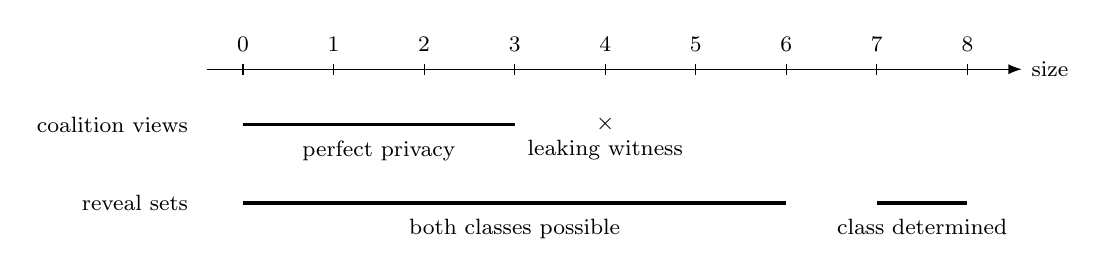
\begin{tikzpicture}[every node/.style={font=\footnotesize},xscale=1.15]
    \draw[-{Latex}] (-0.4,0) -- (8.6,0) node[right] {size};
    \foreach \x in {0,...,8}
      \draw (\x,-0.07) -- (\x,0.07) node[above=1pt] {\x};
    \node[left] at (-0.5,-0.7) {coalition views};
    \draw[very thick] (0,-0.7) -- (3,-0.7)
      node[midway,below=2pt] {perfect privacy};
    \node at (4,-0.7) {$\times$};
    \node[below=2pt] at (4,-0.7) {leaking witness};
    \node[left] at (-0.5,-1.7) {reveal sets};
    \draw[very thick] (0,-1.7) -- (6,-1.7)
      node[midway,below=2pt] {both classes possible};
    \draw[very thick] (7,-1.7) -- (8,-1.7)
      node[midway,below=2pt] {class determined};
  \end{tikzpicture}
  \caption{The recovery ramp $(t,r,n)=(3,7,8)$. The view track shows perfect privacy for
coalitions of at most three positions and leakage for the four-position
witness. The reveal track shows ambiguity through six positions and
determination from seven.}
  \label{fig:ramp}
\end{figure}

The witness coalition shows that the privacy cutoff of three is sharp. Leakage
for reveal sets of sizes four through six reduces to four values, one for each
orbit under $G$. Four-position reveal sets form two orbits of sizes $42$ and
$28$, separated by the classical cross-ratio invariant. Five-position reveal
sets form one orbit, and six-position reveal sets form one orbit.\footnote{The orbit census and the collision counts are kernel-checked
in \path{pgg-smc/instances/pgl27/pgl27_leakage_census.v}, as
\coqin{pgl27\_orbit\_four\_cover}, \coqin{pgl27\_five\_subset\_orbitE},
\coqin{pgl27\_six\_subset\_orbitE}, and the \coqin{pgl27\_collisions}
lemmas.}

Fix an orbit representative $C$ with at least three positions. For either
secret value, restriction of the two deals to $C$ is injective. The
coalition's observation is therefore uniform over $336$ equally likely
possibilities. Let $m$ be the number of observations shared by the two deals.
A shared observation is compatible with both secrets, while every other
observation identifies one secret. Under the uniform secret prior, the
nonshared fraction is $1-m/336$. This is the mutual information with the
secret class in bits. Sharp three-transitivity justifies this identity by a
pen-and-paper argument. The
identity does not apply below three positions, where the true leakage is zero.
The kernel-checked collision counts for the four representatives are $m=96$,
$72$, $36$, and $12$. The corresponding leakage values are $5/7$, $11/14$,
$25/28$, and $27/28$ bits. The committed script
\path{pgg-smc/instances/pgl27/pgl_leakage_targets.py} evaluates these values
from the counts outside the kernel. The four-heart witness represents the
orbit of size $42$ and has leakage exactly $5/7$ bits. A pen-and-paper
relabeling argument extends each value from its representative to the full
orbit because a group element preserves leakage. The formalization does not
include this relabeling-invariance argument.

\subsection{Perfect View and Trace Privacy}

The main uniform-shuffle execution samples $S$ uniformly from $\{0,1\}$. It
deals the fixed representative $D_S$, meaning the chosen encoded deck for
secret $S$.\footnote{The execution distribution is \coqin{pgl27P} and the
representative is the formal orbit encoder \coqin{orbit\_encode}.}
 It then samples an independent shuffle $g\leftarrow
U_G$. Three-transitivity means that any ordered triple of distinct positions
can be moved to any other. This property makes the view independent of the
secret for every coalition $C$ with $\lvert C\rvert\leq3$.

\begin{proposition}[Perfect privacy for the fixed dealer\footnotemark]
\footnotetext{Formalized in \path{pgg-smc/instances/pgl27/pgl27_secrecy.v}
as
\coqin{pgl27\_view\_indep}. The trace counterpart is formalized in
\path{pgg-smc/instances/pgl27/pgl27_trace.v} as
\coqin{pgl27\_coalition\_trace\_secrecy}.}
Assume the uniform Boolean prior, the fixed representative dealer that uses
one chosen deck for each secret, and an independent uniform $\PG$ shuffle.
Then 
\[
  S\mathrel{\perp}V_C
  \quad\text{and}\quad
  H(S\mid T_C)=H(S)
  \qquad\text{for every }\lvert C\rvert\leq3.
\]
\end{proposition}

\begin{example}\label{ex:coalition-view}
Let the dealt secret be $s=0$, so the dealt arrangement is $D_0$. Let the
shuffle be the translation $x\mapsto x+1$, which leaves the point $\infty$
fixed at position seven. Each position then shows the card that $D_0$ places
one position later. The coalition $\{0,1,2\}$ sees the values $(1,2,3)$. For
$s=1$, the same shuffle would show $(1,2,4)$. By
Lemma~\ref{thm:three-transitive}, another shuffle sends the coalition's
positions to positions $1$, $2$, and $4$ of $D_1$. These positions contain the
values $1$, $2$, and $3$. Thus, three observed cards never distinguish the two
secrets. The preceding proposition makes this equality of view distributions
exact.
\end{example}

Two additional dealers test the robustness of the fixed representative choice.
The all-decks dealer checks whether that choice is special. It samples $S$
uniformly. Given $S=s$, it samples a valid arrangement uniformly from class
$s$. It then applies an independent uniform $\PG$ shuffle.\footnote{The all-decks distribution is
\coqin{pgl27P\_alldecks}.}

\begin{proposition}[All-decks perfect privacy\footnotemark]
\footnotetext{Formalized in \path{pgg-smc/instances/pgl27/pgl27_secrecy.v}
as
\coqin{pgl27\_view\_indep\_alldecks}. The trace counterpart is formalized in
\path{pgg-smc/instances/pgl27/pgl27_trace.v} as
\coqin{pgl27\_alldecks\_coalition\_secrecy}.}
Assume the uniform Boolean prior, a dealer that samples a deck uniformly from
the chosen secret class, and an independent uniform $\PG$ shuffle. Then

\[
  S\mathrel{\perp}V_C
  \quad\text{and}\quad
  H(S\mid T_C)=H(S)
  \qquad\text{for every }\lvert C\rvert\leq3.
\]
\end{proposition}

A third dealer samples a valid deck uniformly from the chosen secret class and
applies no later shuffle. I call this law the shuffle-free deck distribution.
Under this law, view independence holds for every Boolean secret prior. The
available executed-trace theorem assumes the uniform Boolean prior. I do not
claim a prior-generic trace theorem.

\begin{proposition}[Shuffle-free deck privacy\footnotemark]
\footnotetext{Formalized in \path{pgg-smc/instances/pgl27/pgl27_secrecy.v}
as
\coqin{pgl27\_view\_indep\_deck\_prior}. The trace counterpart is formalized
in \path{pgg-smc/instances/pgl27/pgl27_trace.v} as
\coqin{pgl27\_deck\_coalition\_secrecy}.}
For any Boolean prior, a deck sampled uniformly from the chosen secret class
gives $S\mathrel{\perp}V_C$ whenever $\lvert C\rvert\leq3$. Thus, the
coalition view is independent of the secret. Under the uniform Boolean prior,
the same dealer also gives $H(S\mid T_C)=H(S)$, so the executed trace
preserves the secret's entropy.
\end{proposition}

Executed correctness gives decoding for the full run. The recovery-ramp
proposition gives the recovery threshold and the four-card leakage witness.
Fixed-dealer privacy gives view and trace privacy through coalition size
three. This makes the four-card witness sharp. Together, these results prove
Theorem A.

\begin{thmA}
For every group element, the $\PG$ instance recovers the secret from all eight
endpoints.\footnotemark{}
 Under the uniform Boolean prior, the fixed representative
dealer that uses one chosen deck for each secret, and an independent uniform
$\PG$ shuffle, the instance has recovery parameters 
\[
  (t,r,n)=(3,7,8),
\]
 and for every
passive coalition $C$ with $\lvert C\rvert\leq3$, 
\[
  S\mathrel{\perp}V_C
  \quad\text{and}\quad
  H(S\mid T_C)=H(S).
\]
\end{thmA}
\footnotetext{This statement is the conjunction of the following formalized
results: \coqin{pgl27\_run\_recovers} in
\path{pgg-smc/instances/pgl27/pgl27_run.v}, \coqin{pgl27\_reveal\_ambiguous}
and \coqin{pgl27\_seven\_reveal\_class} in
\path{pgg-smc/instances/pgl27/pgl27_recovery.v},
\coqin{pgl27\_view\_leak\_k4} and \coqin{pgl27\_view\_indep} in
\path{pgg-smc/instances/pgl27/pgl27_secrecy.v}, and
\coqin{pgl27\_coalition\_trace\_secrecy} in
\path{pgg-smc/instances/pgl27/pgl27_trace.v}.}

Section~\ref{sec:instances} states the trust base for Theorem A.

Theorem A assumes a uniform group element. The next section replaces this
ideal shuffle with a finite generator word and quantifies the resulting error.

\section{Word-Shuffle Approximation of the Uniform-Shuffle Model}\label{sec:mixing}

Section~\ref{sec:model} defines generator words. This section proves a
machine-checked mixing certificate for the finitely generated shuffle. It
shows that evaluating a uniform word gives a distribution close to the uniform
distribution on the group. The letters are group generators, not cuts of the
eight-card row. I do not claim a physical realization of an unobserved letter
application. The main certificate bounds the distance between the executable
and ideal shuffles. The proof then transfers this bound to security
observables. Theorem B states the final bound.

The executable shuffle samples a word over five letters. Three letters are the
projective translation, scaling, and inversion generators. The other two are
the inverses of translation and scaling. Inversion is self-inverse. The fiber
computation steps backward through each letter's inverse, so every inverse
must remain in the alphabet. This symmetric five-letter generator tuple
generates the same group as the original three generators. The fiber count
therefore still concerns the same $336$ group elements.

For word length $L$, the shuffle distribution evaluates a uniform word in
$\{0,1,2,3,4\}^L$. At the length $L=200$ used in Theorem B, the sample space
contains $5^{200}$ words. The proof partitions these words by their evaluated
group element. I call the words that evaluate to $g$ the fiber of $g$. The
$336$ group elements therefore define $336$ fibers. Informally, the
certificate counts how often each group element occurs among the $5^{200}$
words and checks its deviation from the average. For example, at $L=1$, the
translation letter evaluates to $z\mapsto z+1$ and belongs to that group
element's fiber. A computation using binary natural numbers records every
fiber size. The final arithmetic check sums the deviations from the average
size $5^{200}/336$.

\begin{lemma}[Word-shuffle mixing bound\footnotemark]\label{thm:pgl-mixing}
\footnotetext{Formalized in \path{pgg-smc/instances/pgl27/pgl27_mixing.v} as
\coqin{pgl27\_word\_mixing}.}
Let $\mu$ be uniform on the five-letter symmetric generator tuple. Then

\begin{equation}
  \left\lVert \mu^{*200}-U_G\right\rVert_1 \leq 2^{-40}.
  \label{eq:pgl-mixing}
\end{equation}
\end{lemma}

Equation~\ref{eq:pgl-mixing} is a checked mixing certificate. Its inputs are
the five-letter generation theorem, the group order in
Equation~\ref{eq:pgl-order}, the $336$ fiber counts, and the final integer
inequality. The certificate concerns only the distribution of shuffle group
elements.

A coalition observes card endpoints, not group elements. The proof therefore
transfers the bound from group elements to endpoints. The endpoint transfer
maps each permutation to the endpoint of one fixed card. Here $h_\#P$ denotes
the distribution of $h(g)$ when $g$ is sampled from $P$.

\begin{lemma}[Endpoint transfer\footnotemark]\label{lem:endpoint-transfer}
\footnotetext{Formalized in \path{pgg-smc/instances/pgl27/pgl27_mixing.v}
as \coqin{pgl27\_endpoint\_mixing}.}
By the $L_1$ data-processing inequality, for every card position $i$,

\begin{equation}
  \left\lVert
    (g\mapsto \rho(g)i)_\#\mu^{*200}
    -(g\mapsto \rho(g)i)_\#U_G
  \right\rVert_1
  \leq 2^{-40}.
  \label{eq:endpoint-transfer}
\end{equation}
\end{lemma}

The endpoint transfer controls one card position. Transitivity makes the
endpoint distribution under the uniform shuffle uniform on the eight
positions. The privacy theorem also includes the secret variable. The next
lemma forms the product of each shuffle distribution with the same independent
Boolean prior and preserves the $L_1$ bound.

\begin{lemma}[Secret-prior product transfer\footnotemark]\label{lem:product-transfer}
\footnotetext{Formalized in \path{pgg-smc/instances/pgl27/pgl27_mixing.v}
as \coqin{pgl27\_joint\_mixing}.}
Let $\pi$ be any distribution on Boolean secrets. The product distributions
make the secret and shuffle independent, and 
\begin{equation}
  \left\lVert
    \pi\mathbin{\times}\mu^{*200}
    -\pi\mathbin{\times}U_G
  \right\rVert_1
  \leq 2^{-40}.
  \label{eq:product-transfer}
\end{equation}
\end{lemma}

Equations~\ref{eq:endpoint-transfer} and~\ref{eq:product-transfer} apply the
single certificate in Equation~\ref{eq:pgl-mixing} to two additional sample
spaces. Neither equation is a separate mixing certificate.
Equation~\ref{eq:product-transfer} compares a secret prior paired with a
shuffle distribution. It does not yet describe executed runs.

The proof chain establishes proximity of the group distributions, every
single-card marginal, and the product with any secret prior. Transport through
the protocol interpreter then turns the certificate into Theorem B.

\begin{thmB}
Let $\mu$ be uniform on the five-letter symmetric generator tuple.\footnotemark{}

Then 
\[
  \left\lVert \mu^{*200}-U_G\right\rVert_1 \leq 2^{-40}.
\]
 For the fixed representative dealer, every passive coalition
$C$ with $\lvert C\rvert\leq3$, and all secrets $s,s'\in\{0,1\}$, let
$V_C(s,g)$ denote the coalition view at dealt secret $s$ and shuffle $g$. Then

\begin{equation}
  \left\lVert
    (g\mapsto V_C(s,g))_\#\mu^{*200}
    -(g\mapsto V_C(s',g))_\#\mu^{*200}
  \right\rVert_1
  \leq 2^{-39},
  \label{eq:word-view-privacy}
\end{equation}
 and the executed coalition trace satisfies the same bound. Decoding all
eight endpoints returns the dealt secret for every word.
\end{thmB}
\footnotetext{This statement is the conjunction of the following formalized
results: \coqin{pgl27\_word\_mixing} in
\path{pgg-smc/instances/pgl27/pgl27_mixing.v}, and
\coqin{pgl27\_word\_view\_indist}, \coqin{pgl27\_word\_trace\_indist}, and
\coqin{pgl27\_word\_run\_recovers} in
\path{pgg-smc/instances/pgl27/pgl27_word_privacy.v}.}

The proof uses a triangle inequality through the uniform group distribution.
By three-transitivity, the coalition-view distribution under the uniform
shuffle does not depend on the secret. The data-processing inequality applies
the certificate in Equation~\ref{eq:pgl-mixing} to both sides of the triangle.
A companion theorem also gives a bound of $2^{-40}$ for any Boolean prior. It
compares the joint view-and-secret distribution under the word shuffle with
the product of its uniform-shuffle marginals.\footnote{The companion result is
\coqin{pgl27\_view\_mixing}. It is an ideal-proximity statement, not the
privacy definition.}

The word-shuffle privacy results cover only the fixed representative dealer.
The all-decks and shuffle-free dealers use different sample spaces, so the
product-distribution transfer does not apply to them.
Section~\ref{sec:instances} states the trust base for these results.

The $\PG$ argument has four proof layers: construction, recovery, privacy, and
finite-word transfer. Table~\ref{tab:source-index} maps the mathematical
claims used by Theorems A and B to the \Rocq{} results that establish them.

\begin{table}[H]
  \centering
  \small
  \begin{tabular}{p{.40\linewidth}p{.50\linewidth}}
    \toprule
    Mathematical statement & Rocq source name \\
    \midrule
    \multicolumn{2}{@{}l}{\emph{Construction}} \\
    three-transitivity & \coqin{pgl27\_3transitive} \\
    equianharmonic and harmonic orbit counts & \coqin{orbit\_class\_split}, \coqin{orbit\_class\_split\_complement} \\
    encoder returns its orbit class & \coqin{orbit\_encodeK} \\
    group order & \coqin{pgl27\_card} \\
    \midrule
    \multicolumn{2}{@{}l}{\emph{Correctness and recovery}} \\
    executed recovery of the orbit class & \coqin{pgl27\_run\_recovers\_class} \\
    seven cards determine the deck and orbit class &
      \coqin{pgl27\_seven\_reveal\_determines}, \coqin{pgl27\_seven\_reveal\_class} \\
    at most six revealed cards remain ambiguous &
      \coqin{pgl27\_six\_reveal\_ambiguous}, \coqin{pgl27\_reveal\_ambiguous} \\
    four-card view dependence and leakage &
      \coqin{pgl27\_view\_dep\_k4}, \coqin{pgl27\_view\_leak\_k4} \\
    \midrule
    \multicolumn{2}{@{}l}{\emph{Privacy}} \\
    fixed-representative views &
      \coqin{pgl27\_view\_indep}, \coqin{pgl27\_view\_leakage\_le} \\
    fixed-representative traces &
      \coqin{pgl27\_trace\_secrecy}, \coqin{pgl27\_coalition\_trace\_secrecy} \\
    all-decks views and traces &
      \coqin{pgl27\_view\_indep\_alldecks}, \coqin{pgl27\_alldecks\_trace\_secrecy},
\coqin{pgl27\_alldecks\_coalition\_secrecy} \\
    shuffle-free views and traces &
      \coqin{pgl27\_view\_indep\_deck\_prior}, \coqin{pgl27\_deck\_trace\_secrecy},
\coqin{pgl27\_deck\_coalition\_secrecy} \\
    \midrule
    \multicolumn{2}{@{}l}{\emph{Mixing and transfers}} \\
    word mixing certificate & \coqin{pgl27\_word\_mixing} \\
    endpoint and product transfers &
      \coqin{pgl27\_endpoint\_mixing}, \coqin{pgl27\_joint\_mixing} \\
    word view and trace bounds &
      \coqin{pgl27\_word\_view\_indist}, \coqin{pgl27\_word\_trace\_indist} \\
    ideal-proximity companion & \coqin{pgl27\_view\_mixing} \\
    word correctness & \coqin{pgl27\_word\_run\_recovers} \\
    \bottomrule
  \end{tabular}
  \caption{Rocq sources for the $\PG$ results.}
  \label{tab:source-index}
\end{table}

\section{Other Instances and Trust Base}\label{sec:instances}

The framework shows which arguments transfer unchanged across instances and
which require finite or spectral evidence for a specific instance. In addition
to the instances in Sections~\ref{sec:fivecard} and~\ref{sec:pgl}, the $S_5$
and $S_5\times S_5$ instances use the spectral part of the framework.
Table~\ref{tab:instances} records the formally proved result families for all
five instances. The trace-lifting theorem of Section~\ref{sec:framework} is
used unchanged by all five instances. Each instance supplies its own endpoint
bound. Perfect privacy in the table refers to the dealer distribution defined
by that instance. The trace column does not record a second security property.
It records interpreter soundness carrying the same view privacy to the
executed traces of the stated corrupted players.

The PGL instance adds coalition views, coalition traces, the recovery ramp,
and the finite fiber certificate from Section~\ref{sec:mixing}. A coalition
trace collects the executed traces of the corrupted players. The finite fiber
certificate gives exact evidence for finite-word mixing. This mixing result
does not use the imported Rayleigh premise required by the $S_5$ spectral
route.

\begin{table}[t]
  \centering
  \small
  \renewcommand{\arraystretch}{1.15}
  \begin{tabular}{@{}L{.14\linewidth}L{.24\linewidth}
                       L{.25\linewidth}L{.22\linewidth}@{}}
    \toprule
    Instance & Recovery & Perfect privacy & Trace transport \\
    \midrule
    den Boer & five-card AND & one card & one player \\
    Kim & five-card AND & one card & one player \\
    $S_5$ & additive 5-of-5 & fewer than five positions & one player \\
    $S_5\times S_5$ & two additive 5-of-5 shares, each reconstructed from all five positions
      & fewer than five cards in each five-card pile & one player \\
    $\PG$ & $(t,r,n)=(3,7,8)$: privacy threshold, recovery threshold, and player
count & view privacy for coalitions of at most three
      & trace transport for coalitions of at most three \\
    \bottomrule
  \end{tabular}

  \vspace{1ex}

  \begin{tabular}{@{}L{.14\linewidth}L{.40\linewidth}L{.31\linewidth}@{}}
    \toprule
    Instance & Word-shuffle mixing & Trust base \\
    \midrule
    den Boer & exact mixing after one uniform cut & kernel, \coqin{boolp} \\
    Kim & $L=7$, $L_1<2^{-40}$ & kernel, \coqin{boolp} \\
    $S_5$ & word length $L=286$ via a spectral inequality & imported Rayleigh bound for spectral mixing \\
    $S_5\times S_5$ & within-pile decay, exact global $L_1$ floor $1$ because cards never change
piles
      & Rayleigh bound inherited from the $S_5$ instance \\
    $\PG$ & $L=200$, $L_1\leq2^{-40}$ & kernel, \coqin{boolp} \\
    \bottomrule
  \end{tabular}
  \caption{Proof coverage across the five protocol instances. The mixing column uses the
$L_1$ distance defined in Equation~\ref{eq:l1-definition}.}
  \label{tab:instances}
\end{table}

A result's trust base consists of its checker and the axioms on which its
verification depends. In Table~\ref{tab:instances}, \coqin{boolp} is shorthand
for the three classical principles from the MathComp probability stack.
Propositional
extensionality equates logically equivalent propositions. Dependent functional
extensionality equates dependent functions that are pointwise equal.
Constructive indefinite description selects a witness from a proof that one
exists. The $S_5$ and $S_5\times S_5$ mixing bounds also import a
Rayleigh-quotient premise as an axiom. This analytic premise is used only by
the spectral bounds. The $\PG$ group, orbit, cardinality, correctness, and
recovery results are proved without additional local axioms beyond the global
assumptions. The \Rocq{} kernel checks every accepted proof term. It also
checks the results of finite computations performed by the virtual machine,
which evaluates those computations.

The $S_5$ instance represents its secret by additive sharing modulo five. Its
endpoint mixing proof applies a spectral inequality at word length 286. This
inequality controls convergence at that length. The development imports the
required Rayleigh bound as an axiom. The $S_5\times S_5$ instance uses two
disjoint piles and inherits the same Rayleigh premise. The premise gives decay
within each five-card pile. A card never moves between the piles. Its endpoint
distribution therefore cannot converge to the uniform distribution on all ten
positions, which assigns mass to positions in both piles. The formal global
bound approaches the exact $L_1$ floor of one.

\section{Related Work}\label{sec:related}

Den Boer introduced the first card-based cryptographic protocol with the
five-card trick~\cite{denBoer1989,KochFUN2021}. It uses five cards to compute
the AND of two secret bits with perfect security against passive participants.
Later protocols reduced the number of cards and supported other
functions~\cite{MizukiSone2009,MizukiSone2012,KochWalzerHartel2015}.

Koch, Schrempp, and Kirsten use software bounded model checking over encoded
finite protocol spaces~\cite{Koch2019}. Their method searches for protocols
and checks finite lower bounds. The \Rocq{} formalization instead proves
reusable lemmas for group actions, execution, privacy, and mixing. The Kim
instance also connects a biased shuffle model with a concrete word-shuffle
bound~\cite{KimCetinkaya2025}.

Shinagawa specifies a card protocol through a deck and a set of operations in
a unified model~\cite{Shinagawa2021}. This model covers binary, regular
polygon, and dihedral cards. Shinagawa varies the card type and allowed
physical operations. This paper instead varies the finite group, permutation
action, shuffle distribution, and reconstruction map. It connects these
parameters with executable traces and machine-checked privacy and mixing
results.

Mizuki and Shizuya's abstract-machine model provides the field's standard
operational semantics~\cite{MizukiShizuya2014}. It fixes the sequences of
shuffles, turns, and permutations that a protocol may apply. This paper's
interpreter provides the analogous execution model for group-parametric
protocols. It draws the shuffle from a word distribution over the group's
generators.

Work on closed shuffles and graph automorphisms provides a physical point of
comparison for group-based shuffle models. Miyamoto and Shinagawa realize a
uniformly chosen graph automorphism with pile-scramble
shuffles~\cite{MiyamotoShinagawa2022}. Shinagawa and Miyamoto extend this
construction to graphs and hypergraphs and apply it to cyclic group
shuffles~\cite{ShinagawaMiyamoto2023}. These physical protocols implement
structured uniform shuffle groups exactly. This paper's word approach offers a
different tradeoff. A pile-scramble realization samples its group uniformly in
one physical procedure, while a word shuffle repeats elementary moves and
incurs a kernel-certified $L_1$ error of $2^{-40}$. That line of work provides
unobserved physical realizations for structured shuffles. I leave open whether
the five $\PG$ letters admit such realizations. The eight-card instance also
has a larger deck vocabulary than two-symbol encodings. It stores a Boolean
secret in the arrangement of eight pairwise distinct cards, whereas committed
formats store one bit in two two-symbol cards~\cite{MizukiSone2009}. Broader
results show what physical shuffle models can support. A single uniform closed
shuffle can compute any Boolean circuit~\cite{ShinagawaNuida2021}. A later
compiler maps simple finite-runtime card protocols to private
simultaneous-message protocols~\cite{ShinagawaNuida2025}. Because this paper
uses an approximate word shuffle, the next comparison concerns the formal
tools used to certify its mixing bound.

Machine-checked probability libraries provide results that can support mixing
arguments. Karayel formalizes expander graphs, Cheeger's inequality, and
random-walk tail bounds in Isabelle/HOL~\cite{Karayel2023}. Barthe,
Gr\'egoire, Hsu, and Strub develop a relational program logic for couplings
and apply it to rapid-mixing examples~\cite{BartheEtAl2017}. Standard
mathematical treatments connect spectral information with convergence of
finite Markov chains~\cite{LevinPeresWilmer2009}. The $\PG$ proof uses exact
fiber counting instead. It counts the fibers at one finite word length and
checks the resulting integer inequality. This method gives a concrete bound
without requiring a general spectral development.

Proof-assistant frameworks for cryptography include CertiCrypt, CryptHOL, and
SSProve~\cite{CertiCrypt,CryptHOL,SSProve}. They support program semantics,
probabilistic reasoning, or modular cryptographic proofs at different levels.
This paper proves information-theoretic bounds rather than game-based
reductions. It therefore uses MathComp and infotheo for finite algebra,
probability, independence, and entropy~\cite{MathComp,InfoTheo}. The earlier
FORTE development provides the interpreter and trace semantics used
here~\cite{WengEtAl2025}. This paper extends those semantics with
group-parametric card shuffles and coalition traces.

\section{Conclusion and Future Work}\label{sec:conclusion}

I presented a group-parametric \Rocq{} framework for card-based protocols and
instantiated it with the action of $\PG$ on eight positions. Theorem A proves
executed correctness, recovery parameters $(3,7,8)$, and perfect view and
trace privacy for coalitions of at most three players under the uniform group
distribution. The tuple $(3,7,8)$ gives the privacy threshold, recovery
threshold, and total-player count. These security results assume a uniform
Boolean prior, the fixed representative dealer, passive adversaries, and the
dealer distributions in Section~\ref{sec:model}. The verifier learns the
secret. Theorem~\ref{thm:generic-privacy} requires only a three-transitive
action, a fixed encoding into decks of distinct cards, and the uniform group
distribution. It therefore applies to any instance that supplies these three
inputs.

For a finite shuffle implementation, Theorem B gives an $L_1$ distance of at
most $2^{-40}$ after 200 generator letters. The same bound holds for every
single-card endpoint and for the product with any Boolean secret prior. The
approximate coalition-view and executed-trace bounds are $2^{-39}$. The
word-shuffle model therefore replaces the ideal uniform shuffle at a
quantified, machine-checked cost.

The word-shuffle security results leave two direct extensions open. First,
converting the $L_1$ bound into a conditional-entropy bound uses classical
mathematics. Continuity of entropy in total variation is the Fannes
inequality~\cite{Fannes1973,CsiszarKorner2011}. Only its formalization remains
open here because the underlying probability library does not yet provide it.
Second, the all-decks and shuffle-free dealers need word-shuffle mixing
statements on their own sample spaces. Two broader directions would extend the
framework. Connecting bounded-width branching programs with group-based card
protocols through Barrington's theorem~\cite{Barrington1989,DvorakKoucky2021}
would make the workshop abstract's $\mathrm{NC}^1$ compilation proposal
precise. Further work should also add active and compositional security by
building on models for active card protocols~\cite{KochFUN2021}. A separate
proof-completeness issue concerns the quantitative leakage for reveal sets of
four through six cards. Section~\ref{sec:exact} settles these values at the
current trust level. The orbit census and collision counts are kernel-checked,
and a committed script evaluates the four values from these counts. Two
kernel-level steps remain open. One is a proof of the mutual-information
identity. The other is a proof of the orbit-invariance step that extends each
value from its representative.

\subsubsection*{Acknowledgements and AI-use statement.}

I used LLM-generated proof scripts and documentation drafts under human
specification and review. I remain responsible for the mathematical
specification, claims, citations, and final text.

\subsubsection*{Disclosure of Interests.}

I declare no competing interests.

\bibliographystyle{splncs04}
\bibliography{references}
\end{document}
